\documentclass[12pt,a4paper]{article}
\usepackage[utf8]{inputenc}
\usepackage[T1]{fontenc}
\usepackage[portuguese]{babel}
\usepackage{amsmath}
\usepackage{amsfonts}
\usepackage{amssymb}
\usepackage{graphicx}
\usepackage{subcaption}
\usepackage{booktabs}
\usepackage{hyperref}
\usepackage[left=1.0cm, right=1.00cm, top=2.00cm, bottom=2.00cm]{geometry}
%\author{Guilherme Bertoldo e Jonas Joacir Radtke}
\title{Documentação\\ rRocket v1.5.6}
\bibliographystyle{plain}
\begin{document}
	\maketitle

\section{Introdução}

Esta é uma versão preliminar da documentação do rRocket que servirá de base para a elaboração do artigo. O texto da introdução deverá:
\begin{itemize}
	\item Apresentar a necessidade de altímetros com capacidade de dois eventos de ejeção de paraquedas, contextualizando a disponibilidade deste tipo de equipamento no Brasil.
	\item Descrever a proposta de altímetro de projeto aberto (\textit{open hardware} e \textit{open software}) do rRocket. 
	\item Alertar o usuário sobre a necessidade de aplicação de regras de segurança no lançamento de minifoguetes, destacando que nenhum sistema eletrônico é infalível e que, em caso de falha do rRocket, deve-se prever um local em que a queda do minifoguete não cause danos à vida e ao patrimônio. Isentar os autores de qualquer responsabilidade sobre acidentes que venham a ocorrer.
\end{itemize}


\section{Modelagem}

Para projetar o controle do sistema de recuperação, é necessário conhecer previamente o comportamento típico da trajetória de minifoguetes e as situações adversas que podem ocorrer.

\subsection{Trajetória ideal}
Em um cenário ideal, a componente vertical $h$ da trajetória do minifoguete varia com o tempo $t$ de acordo com a Fig.~\ref{fig:trajectoryA}. Entre A e B, o minifoguete aguarda o lançamento em repouso. Em B ocorre a ignição do motor e o foguete inicia o movimento acelerado. Entre B e C ocorre a queima do propelente (fase propulsada). Entre C e E ocorre o movimento balístico, com apogeu no ponto D. No ponto E ocorre a implantação do paraquedas auxiliar. Entre E e F, o minifoguete cai com velocidade constante. No ponto F ocorre a implantação do paraquedas principal. Entre F e G, o minifoguete cai com velocidade constante, porém, menor do que no intervalo de E a F. No ponto G o minifoguete entra em repouso e permanece assim até o ponto H. 
\begin{figure}[!ht]
	\centering
	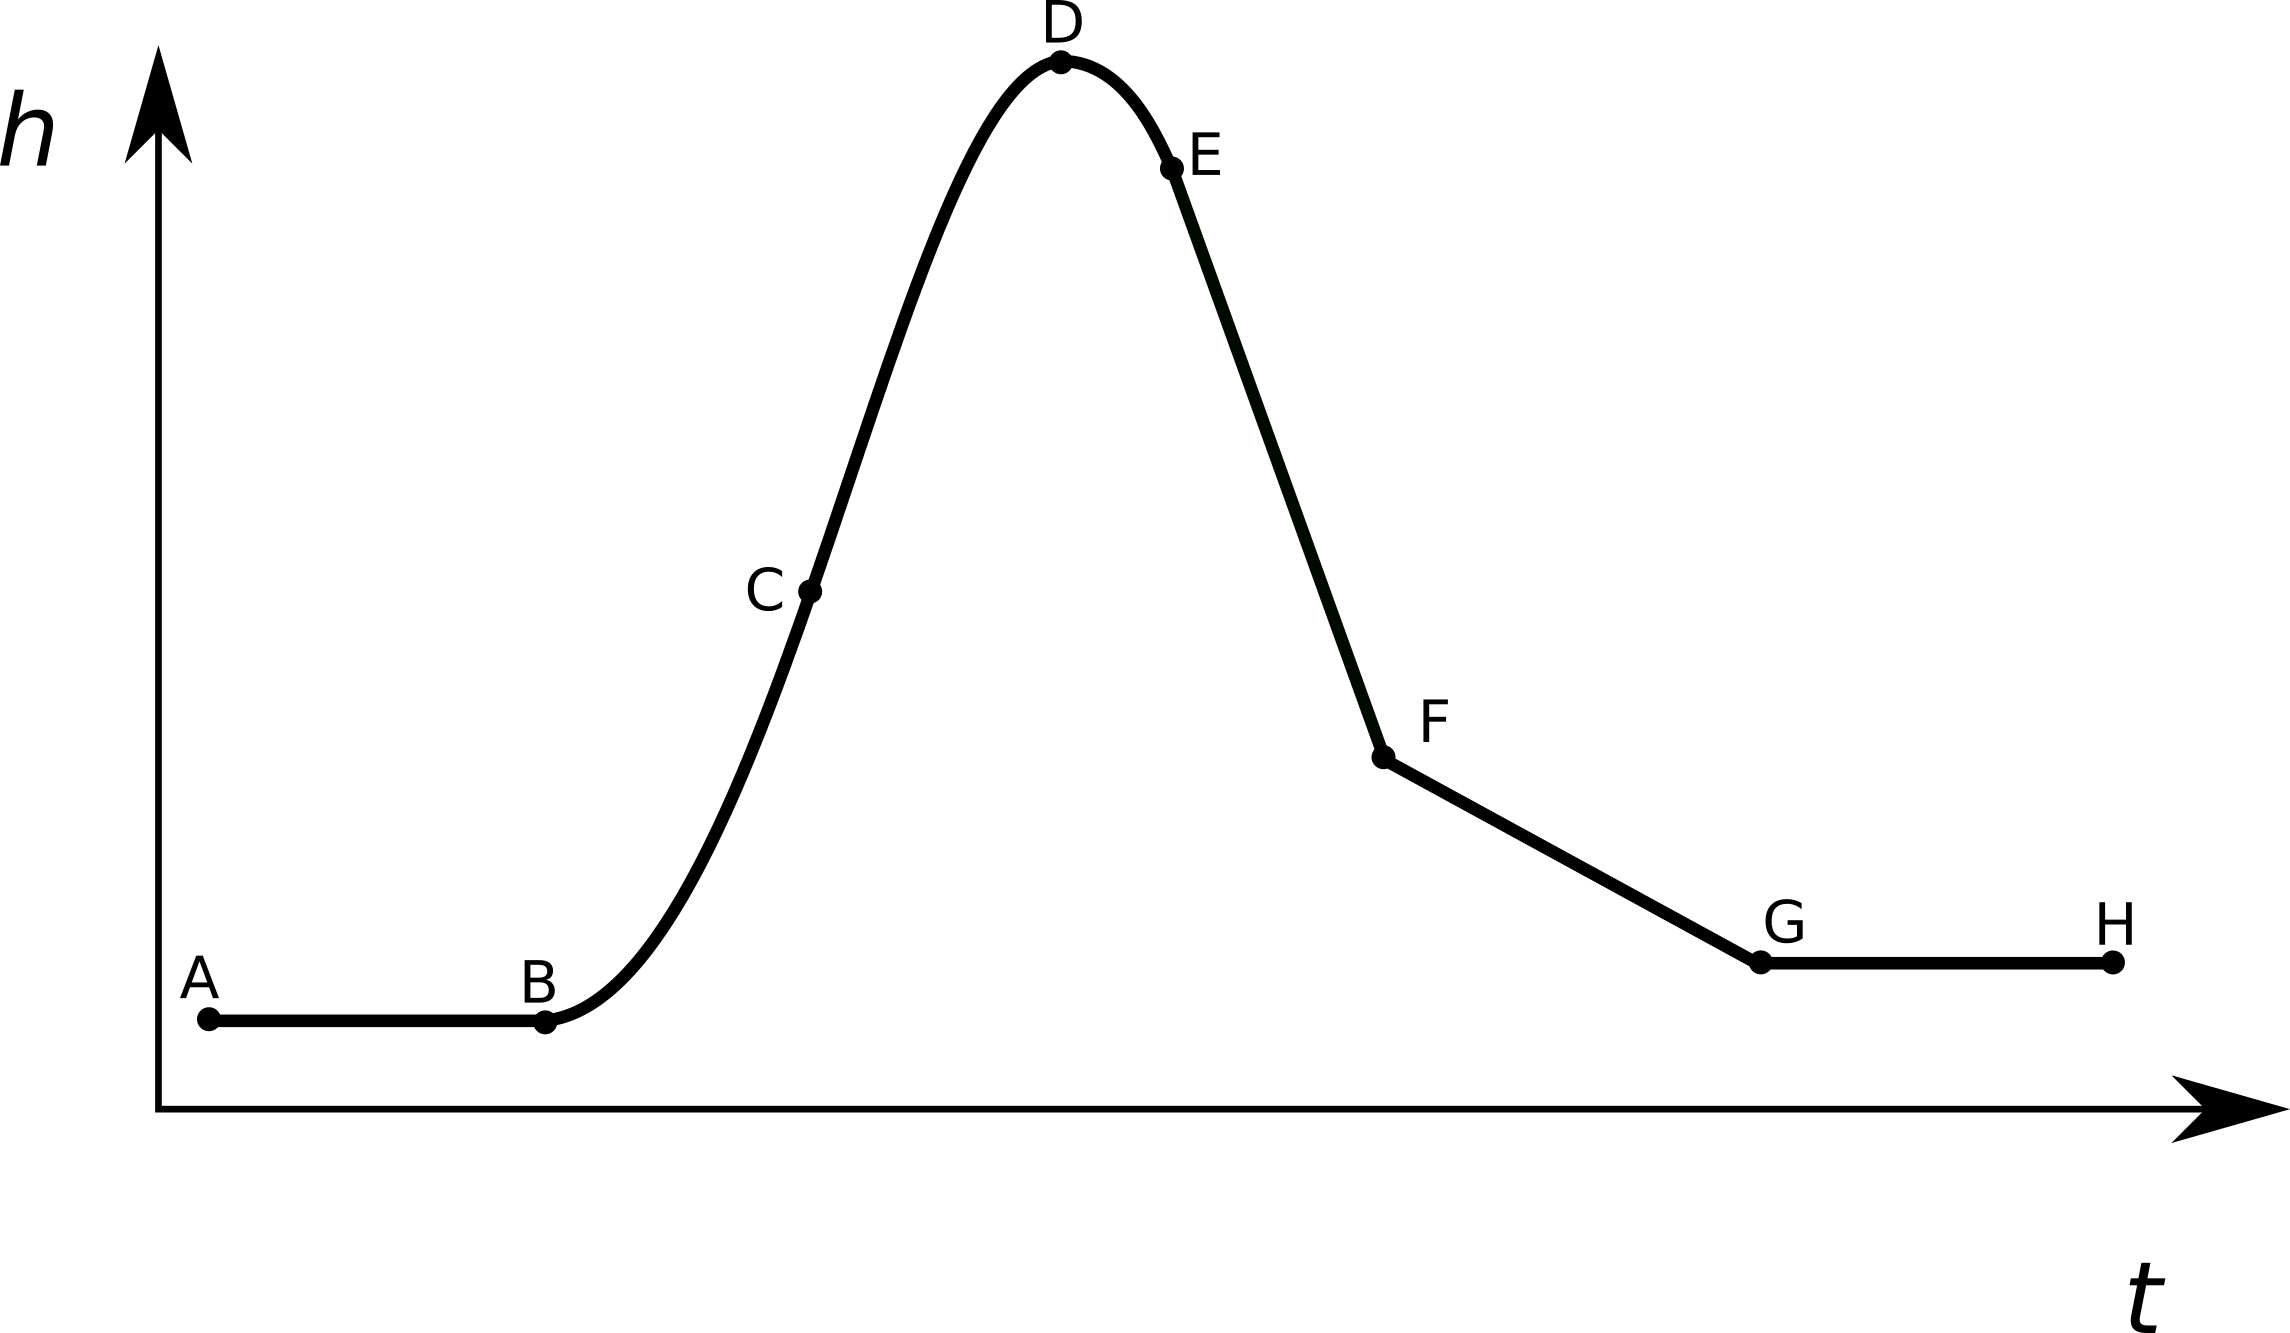
\includegraphics[width=0.6\textwidth]{./fig/trajectoryA}
	\caption{Trajetória típica em um voo de minifoguete com recuperação em dois estágios.}
	\label{fig:trajectoryA}
\end{figure}

\subsection{Adversidades}
\label{sec:adversities}

As principais adversidades relacionadas ao sistema de recuperação que devem ser levadas em conta no \textit{software} de controle do altímetro, no manuseio do altímetro e na montagem do minifoguete são listadas abaixo: 
\begin{enumerate}
	\item Os sistemas de recuperação baseados em barômetro relacionam a pressão e a temperatura ambiente à altitude. Para que $h$ seja determinado corretamente a partir da altitude registra pelo barômetro, é necessário garantir que a pressão e a temperatura ambientes sejam as mesmas no interior do minifoguete. Esta condição é satisfeita se houver furos na fuselagem do minifoguete com diâmetros adequados e em posições adequadas\cite{PerfectFlite} que permitam a equalização da pressão interna à externa.
	
	\item O sensor de pressão fornece $h$ com incerteza $\pm U_h$. O ruído em $h(t)$ é particularmente perceptível entre A e B e entre G e H, como ilustrado na Fig~\ref{fig:adverseA}.
	\item O sistema de recuperação é ligado em uma altitude e lançado em outra. Durante o transporte do local de montagem para o local de lançamento pode ocorrer a detecção de voo (Fig~\ref{fig:adverseE}).
	\item O sistema de recuperação fica ligado por tempo suficientemente grande para que as condições atmosféricas mudem e, consequentemente, haja alteração no registro de $h$, causando detecção errada de voo (Fig~\ref{fig:adverseD}).
	\item Durante o voo do minifoguete, é possível que ocorram oscilações na leitura da pressão devido à instabilidade na trajetória, vibrações, rajadas de vento laterais, que causam perturbações no escoamento.  Aumentos de pressão  também podem ocorrer quando o foguete ultrapassa a velocidade do som ou imediatamente após o lançamento devido à aceleração. As oscilações na pressão causam variações falsas em $h$, como ilustrado nos pontos P e Q da Fig.~\ref{fig:adverseB}, que podem indicar uma situação de queda e levar à implantação prematura dos paraquedas.
	\item Durante a montagem do minifoguete, com o sistema de recuperação ligado, é possível que variações de pressão causem detecção de voo (Fig~\ref{fig:adverseF}).
	\item A altitude de pouso é geralmente diferente da altitude de decolagem.
	\item Reinicialização do dispositivo em voo.
	\item Falha de inicialização de componentes críticos (barômetro e acionador de paraquedas).
	\item Falha de funcionamento de componentes críticos em voo.
	\item Falha de implantação de paraquedas.
\end{enumerate}

\begin{figure}[!ht]
	\centering
	\begin{subfigure}{0.48\textwidth}
		\includegraphics[width=\textwidth]{./fig/trajectoryB}
		\caption{Ruídos na leitura da pressão.}
		\label{fig:adverseA}
	\end{subfigure}
	\begin{subfigure}{0.48\textwidth}
	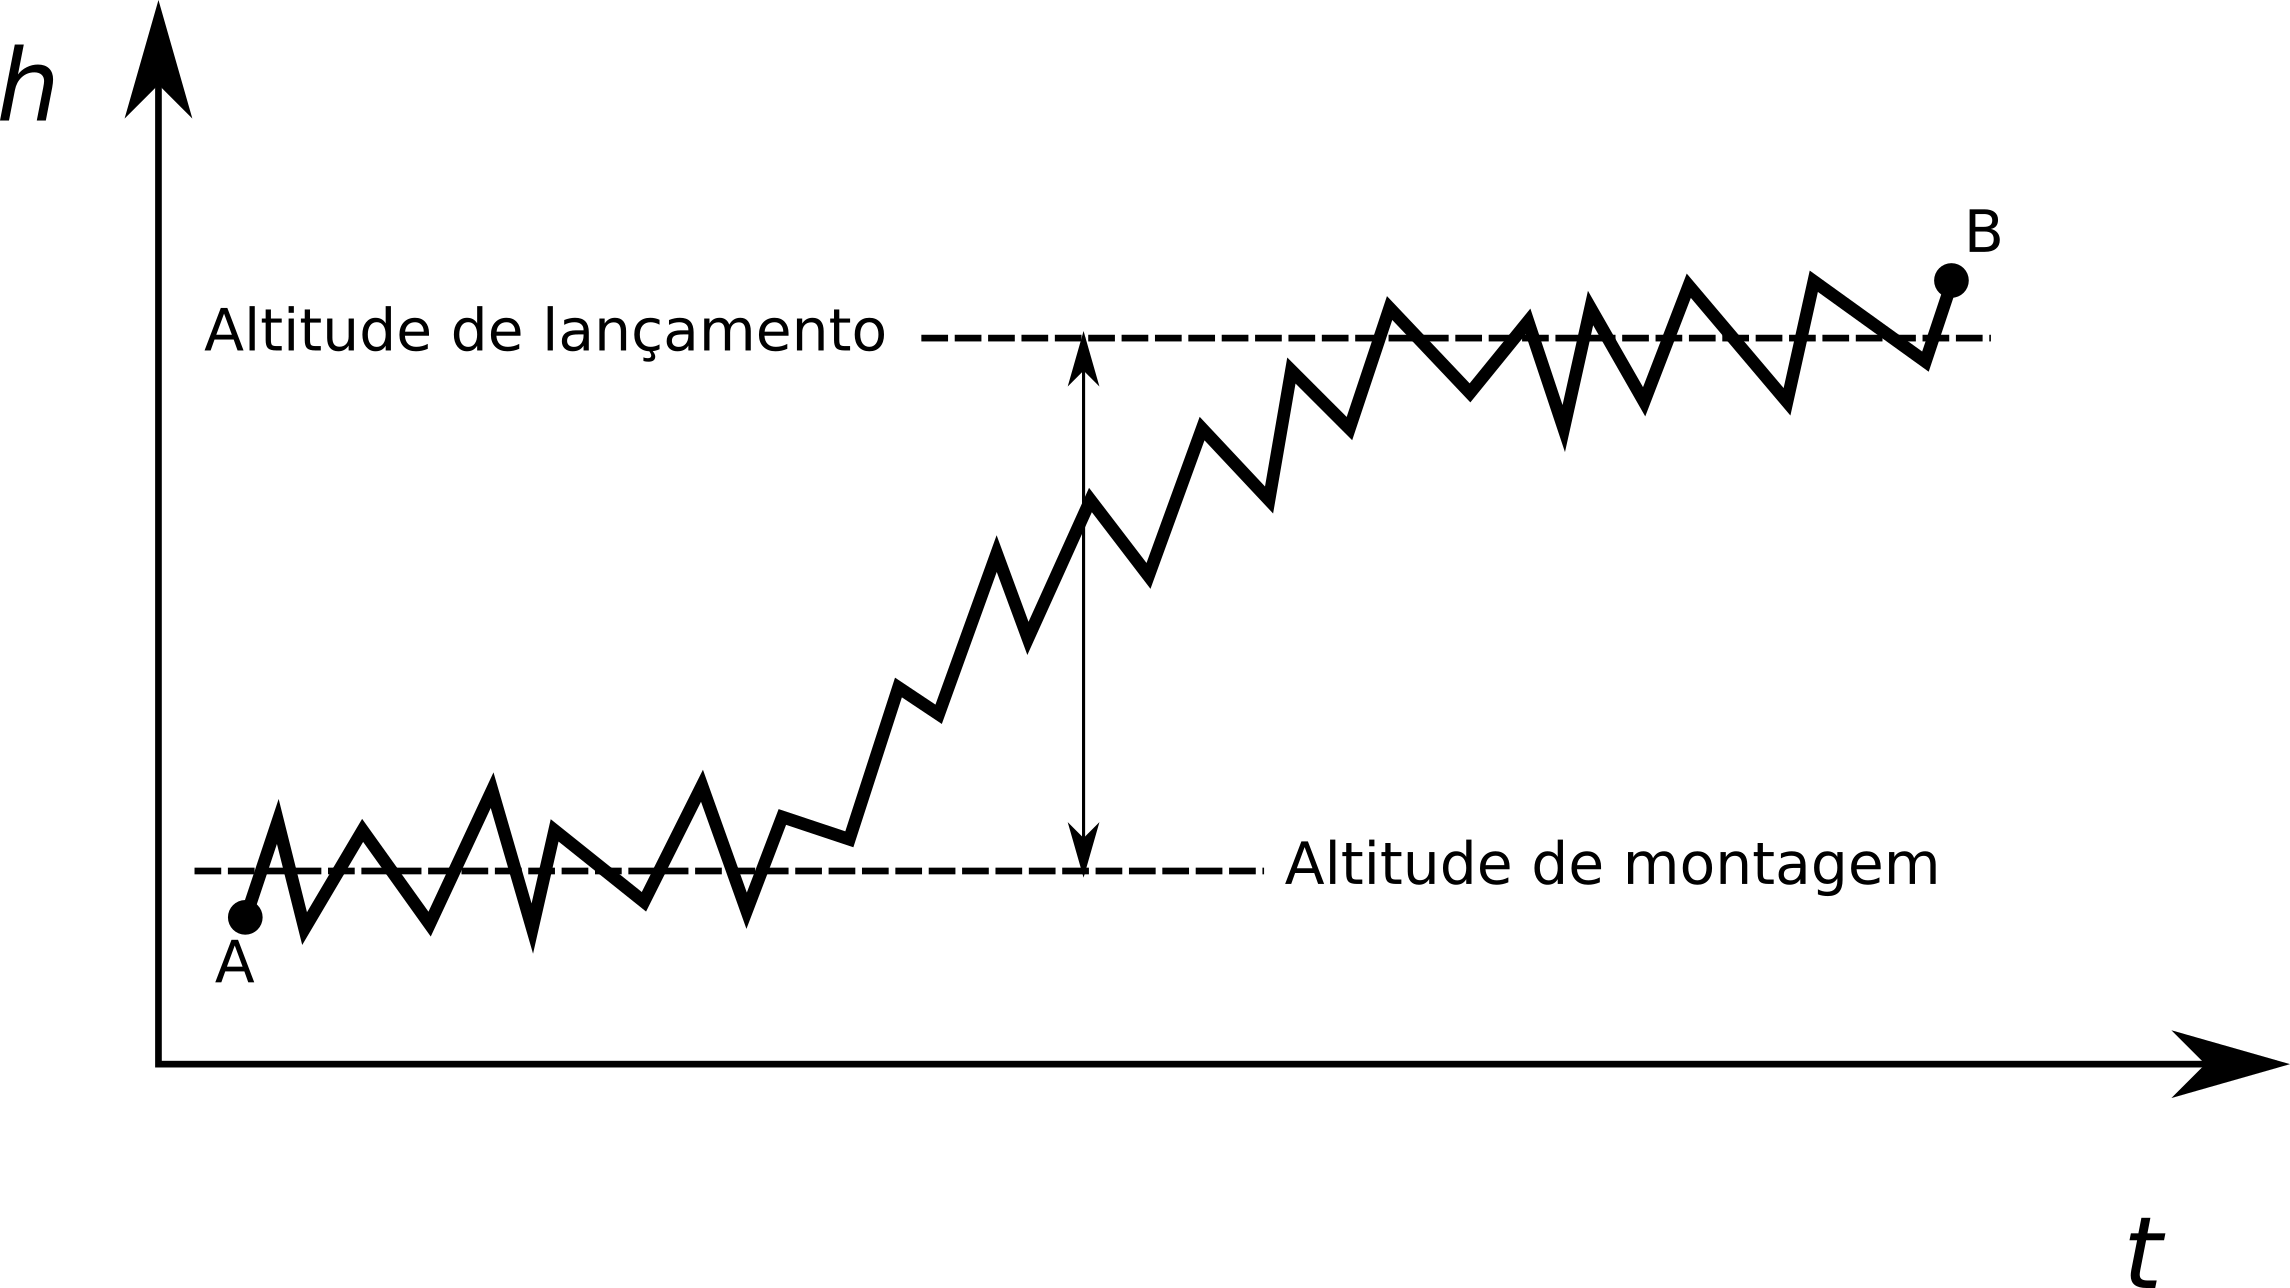
\includegraphics[width=\textwidth]{./fig/trajectoryE}
	\caption{Transporte do dispositivo ligado.}
	\label{fig:adverseE}
	\end{subfigure}
	\begin{subfigure}{0.48\textwidth}
	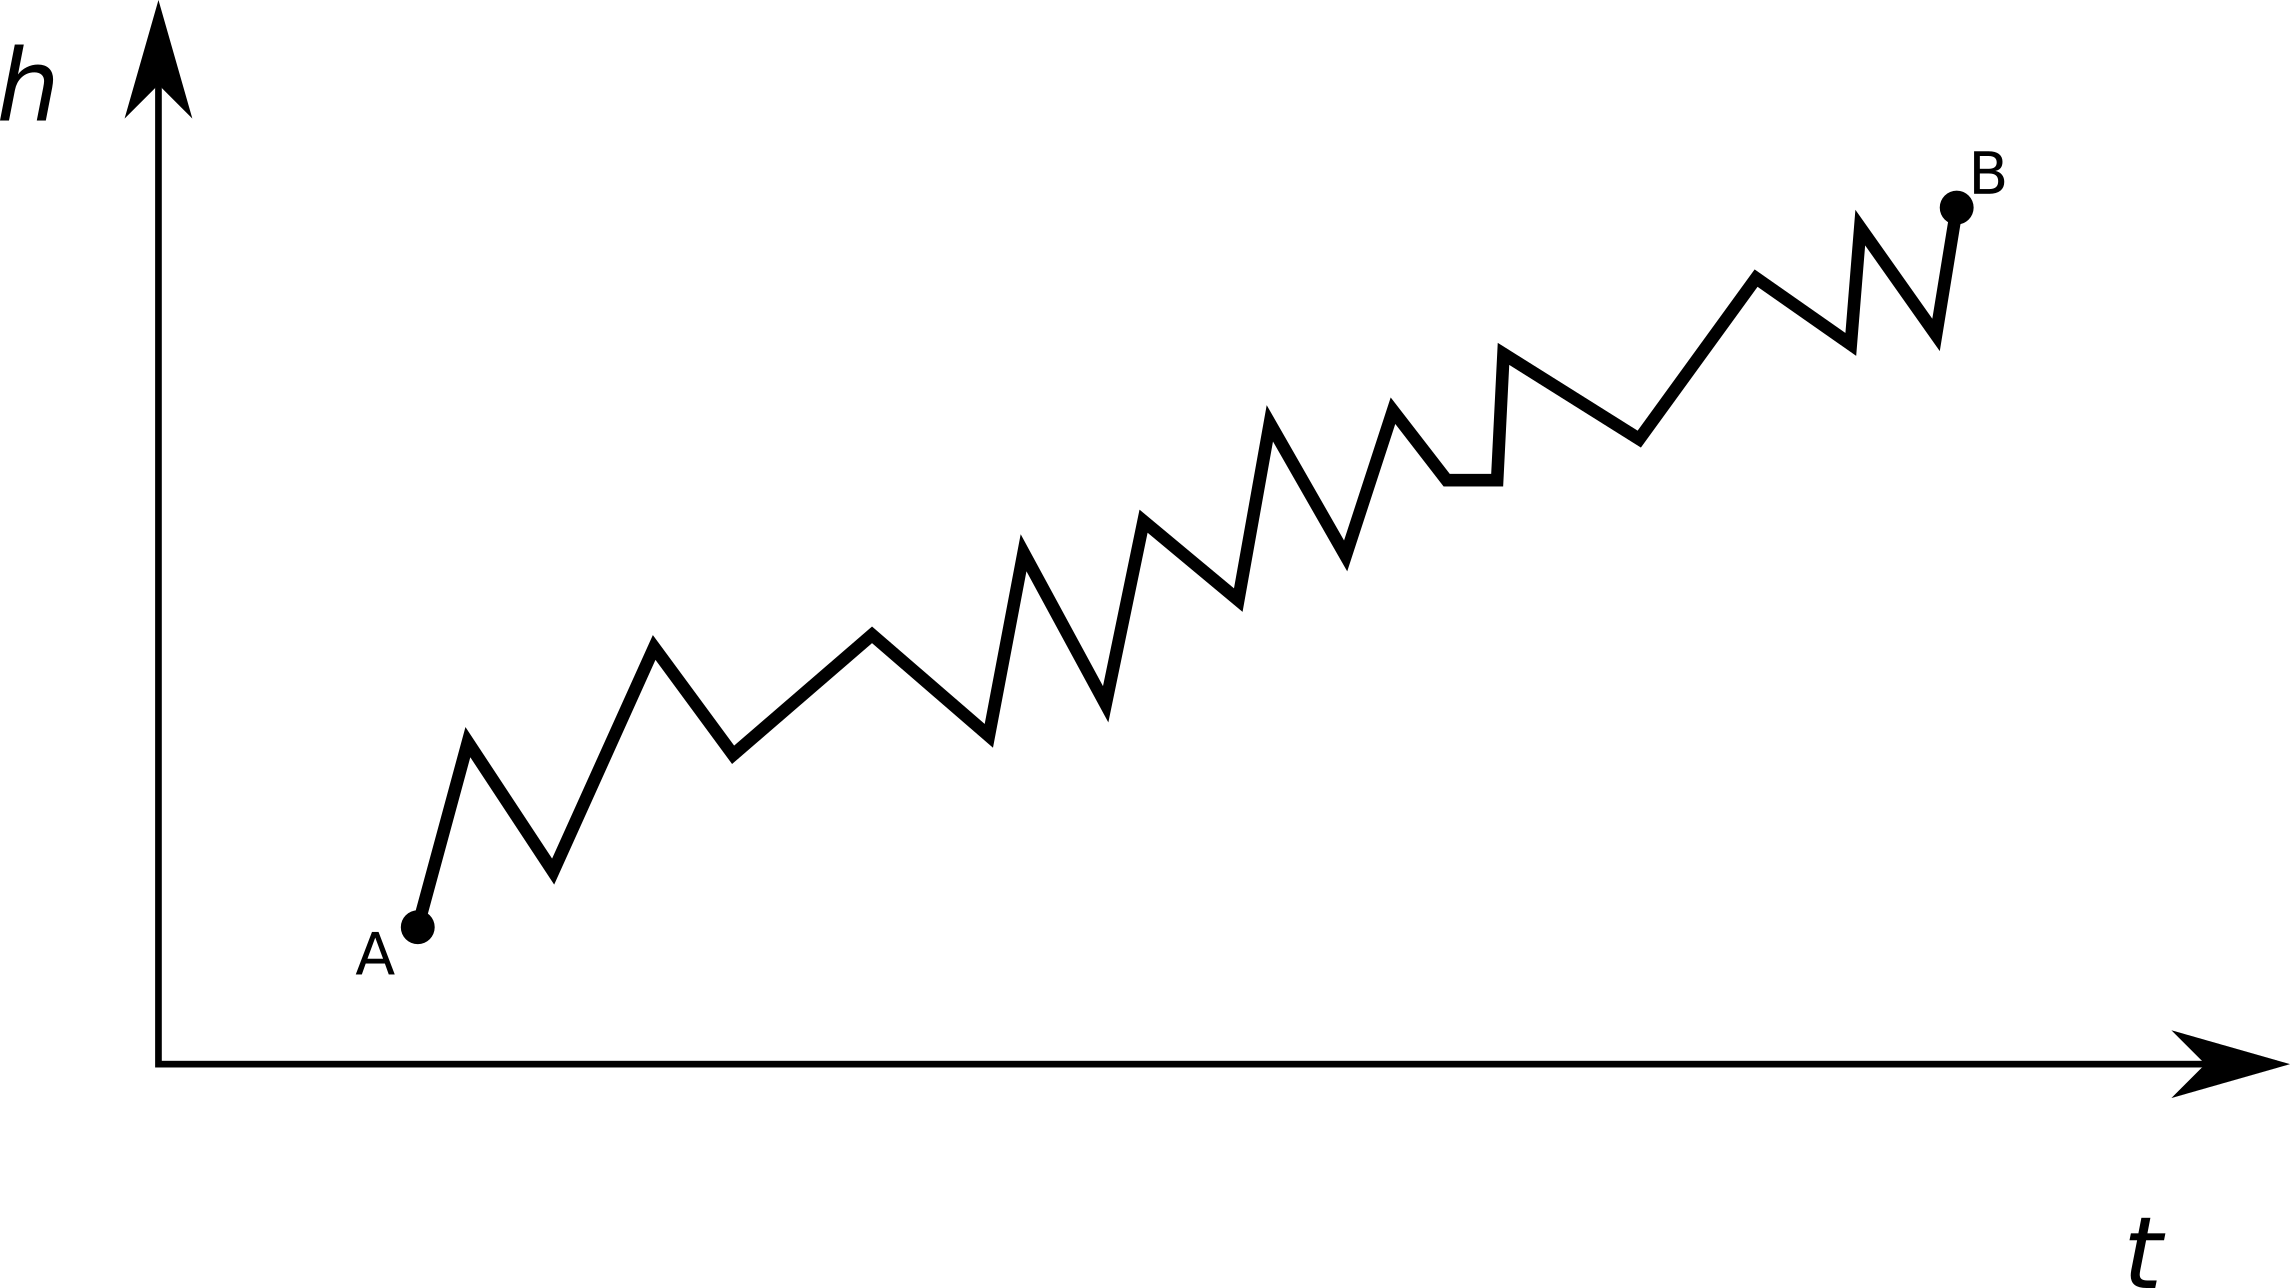
\includegraphics[width=\textwidth]{./fig/trajectoryD}
	\caption{Mudança das condições atmosféricas.}
	\label{fig:adverseD}
	\end{subfigure}
	\begin{subfigure}{0.48\textwidth}
		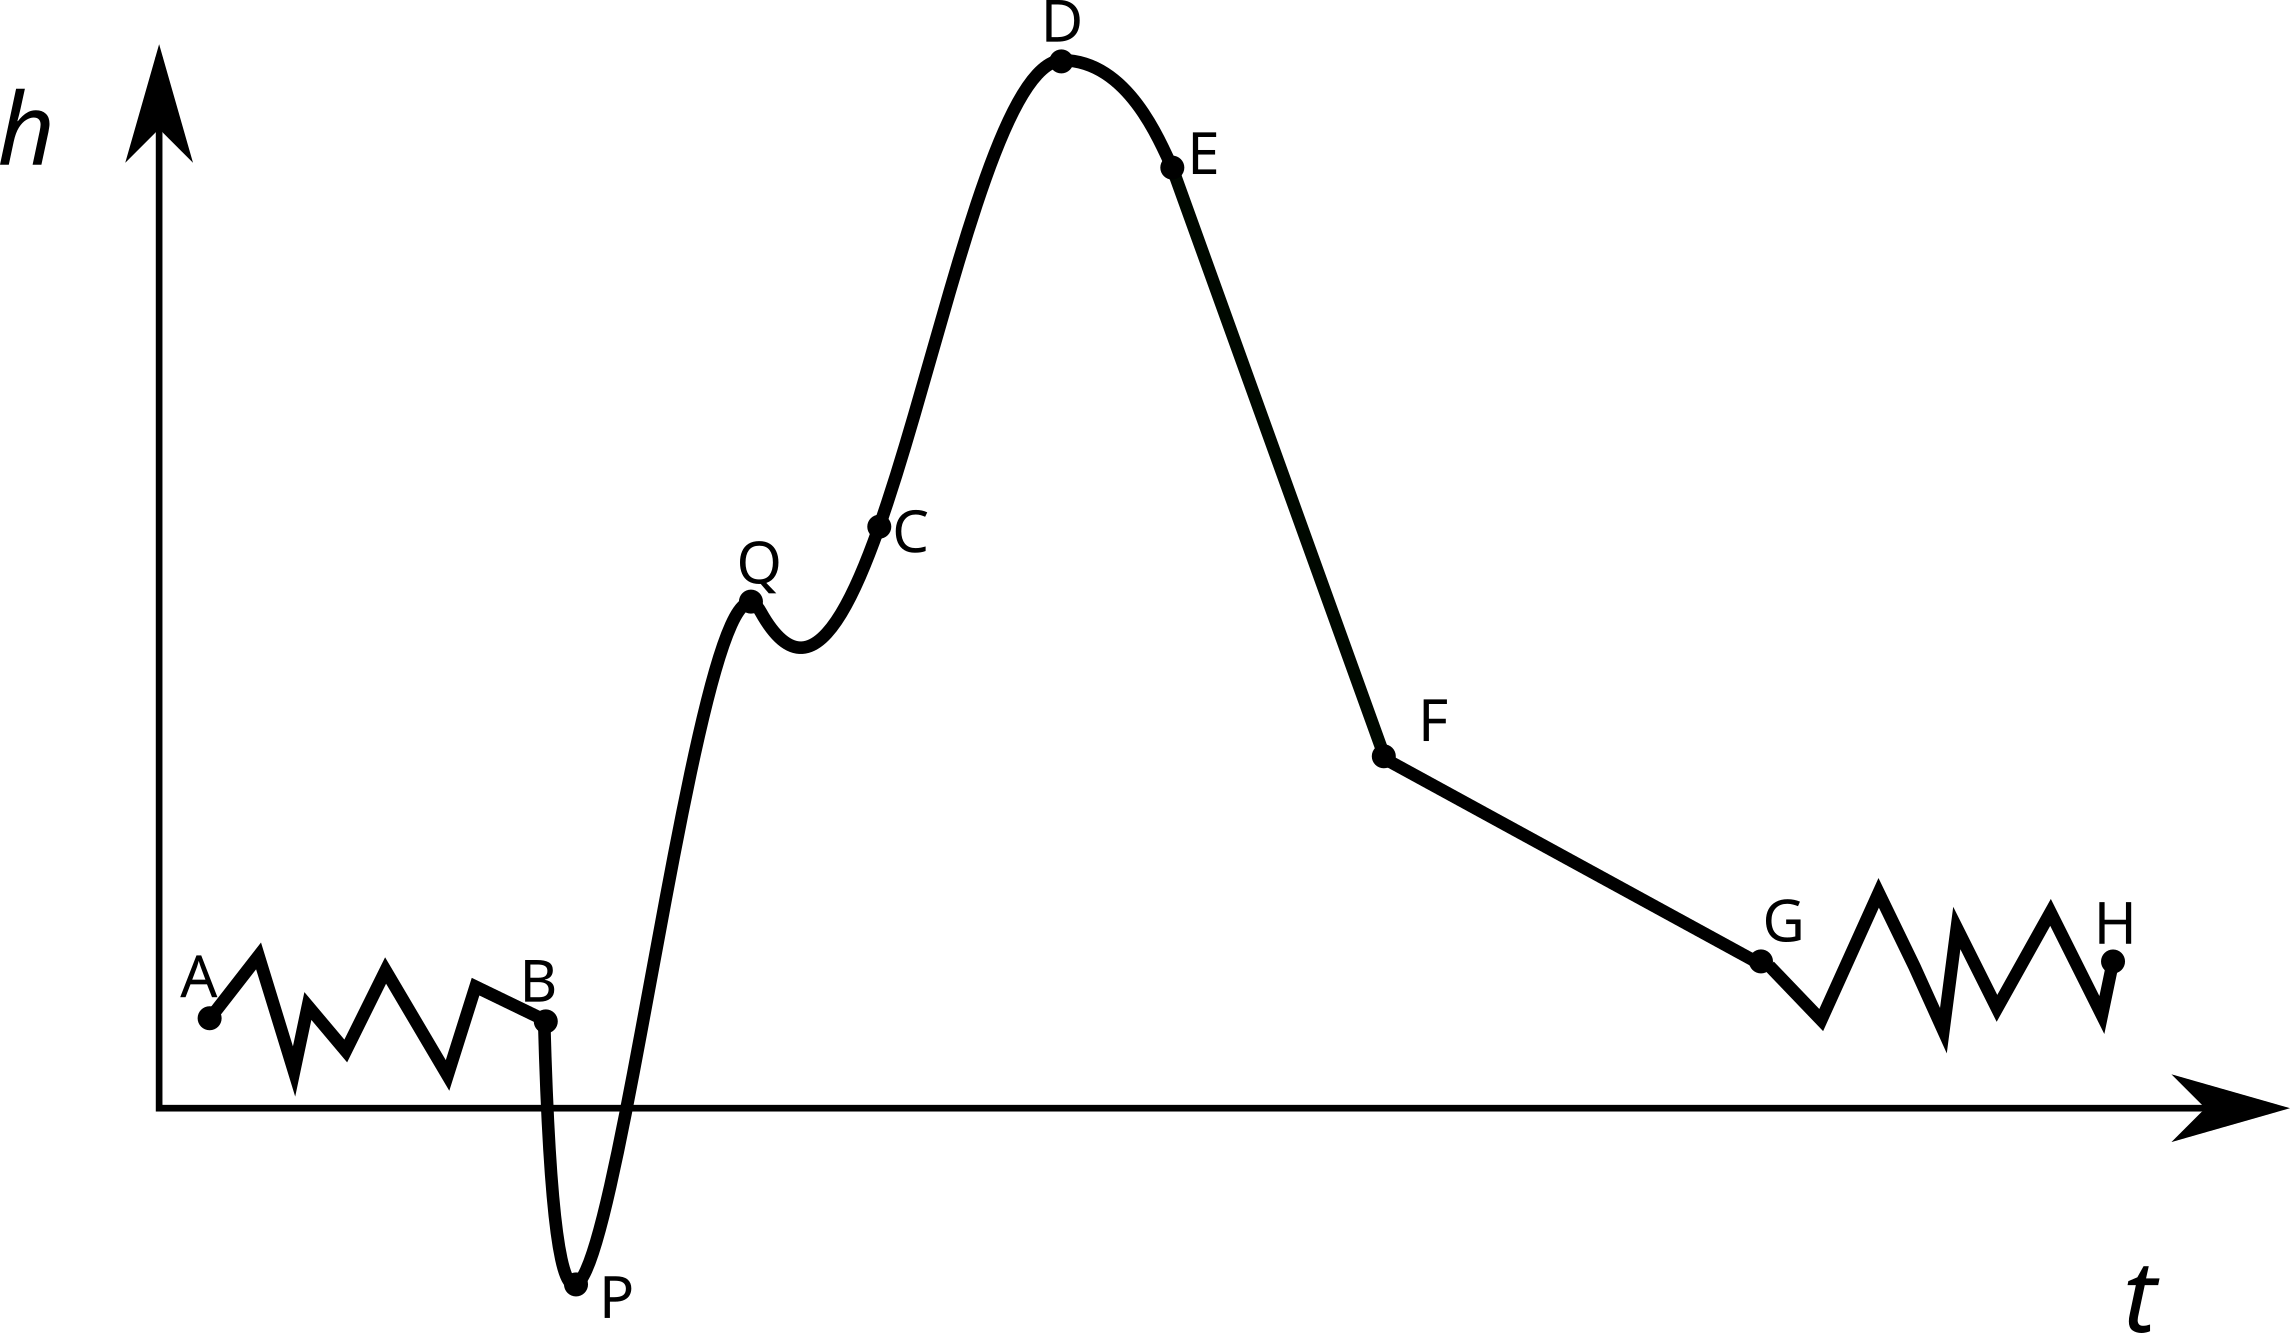
\includegraphics[width=\textwidth]{./fig/trajectoryC}
		\caption{Variação abrupta de pressão.}
		\label{fig:adverseB}
	\end{subfigure}
	\begin{subfigure}{0.48\textwidth}
	\includegraphics[width=\textwidth]{./fig/trajectoryF}
	\caption{Variação de pressão na montagem.}
	\label{fig:adverseF}
	\end{subfigure}
	\caption{Situações adversas na leitura do sensor de pressão.}
	\label{fig:adverse}
\end{figure}

As situações adversas 1 e 6 exigem cuidado do usuário na construção e na montagem do minifoguete. As situações 2 a 8 são levadas em consideração através dos critérios de detecção de eventos de voo (Seç.~\ref{sec:flightevents}). As situações 8 e 9 são consideradas no algoritmo do sistema de recuperação (Seç.~\ref{sec:software}). As situações 10 e 11 não podem ser resolvidas pelo altímetro, embora o algoritmo esteja preparado para mitigar a situação 11, fazendo um número configurável tentativas de acionamento de cada paraquedas.

\subsection{Critérios de detecção de eventos de voo}
\label{sec:flightevents}

Neste documento, são denominados eventos de voo (i) a decolagem, (ii) o apogeu, (iii) a queda, (iv) a altitude de lançamento de paraquedas e (v) o pouso. Para determiná-los, considere que $h(t)$ seja medido com período $T$ e que as últimas $N+1$ medidas sejam armazenadas em um vetor $h_k\quad (1\le k \le N)$.
%Launch Detect Altitude 160 feet to 300

As condições de decolagem, apogeu e queda são baseadas na componente vertical $v_y$ da velocidade. No entanto, como mencionado na Seç.~\ref{sec:adversities}, as medidas de $h$ estão sujeitas à incerteza de leitura do barômetro $U_h$ e às oscilações na pressão, que podem causar falsos eventos de voo. 

Uma das formas de suavizar oscilações é o uso de média. Por isso, neste documento, para calcular o valor médio $\bar{v}_y$ da componente vertical da velocidade $v_y$ utiliza-se a média móvel de $h$. O vetor $h_k$ é dividido em duas partes e, então, calcula-se $h_B$ e $h_F$, que são os valores médios de $h_k$ na primeira e segunda metade do vetor, respectivamente.   

Utilizando a regra dos trapézios, $h_B$ e $h_F$ são calculados como
\begin{equation}
	h_B=\frac{1}{N/2}\left[\frac{h_0+h_{N/2}}{2}+\sum_{k=1}^{N/2-1}h_k\right], \quad h_F=\frac{1}{N/2}\left[\frac{h_N+h_{N/2}}{2}+\sum_{k=1}^{N/2-1}h_{N-k}\right].
\label{eq:haverage}
\end{equation}

Uma vez conhecidos $h_B$ e $h_F$, $\bar{v}_y$ é obtido por diferenças finitas como
\begin{equation}
\bar{v}_y=\frac{h_F-h_B}{NT/2}.
\end{equation}

Note que as médias (\ref{eq:haverage}) são calculadas no período $\tau=NT/2$. A capacidade de suavização da média é mais efetiva quando $T_p \ll \tau$, onde $T_p$ é período das perturbações. O valor de $\tau$, portanto, deve ser suficientemente grande para suavizar as oscilações e suficientemente pequeno para captar adequadamente a dinâmica do voo. 

Com base em $h_k$ e no procedimento de suavização da velocidade descrito acima, os critérios de detecção de eventos de voo são:
\begin{itemize}
	\item \textbf{Condição de decolagem}:
	\begin{equation}
	\bar{v}_y>v_\text{liftoff},
	\end{equation}
	onde $v_\text{liftoff}$ é a velocidade mínima para detectar a decolagem. $v_\text{liftoff}$ deve ser suficientemente grande para que perturbações na pressão não causem acionamento prematuro do sistema de recuperação, mas não tão grande para que o lançamento não seja detectado. Sugere-se  
	\[20~\text{m/s} \le v_\text{liftoff}\le 40~\text{m/s}.\]
	
	Note que o uso do procedimento de suavização de velocidade e a condição de decolagem proposta evitam as situações adversas 2 a 6.
	\item \textbf{Condição de apogeu}:
	\begin{equation}
	\bar{v}_y<v_\text{apogee},
	\end{equation}
	onde $v_\text{apogee}$ é a velocidade para detecção de apogeu. Em uma trajetória suave, o apogeu ocorre em $v_y=0$. No entanto, devido ao atraso causado pelo processo de suavização no cálculo da velocidade, admite-se que o apogeu ocorre em uma velocidade um pouco maior que zero. Sugere-se 
	\[0 \le v_\text{apogee}<\frac{gNT}{3}\qquad \text{e} \qquad v_\text{apogee} \ll v_\text{liftoff},\]
	onde $g$ a aceleração gravitacional. Além disso, é fundamental que
	\[ v_\text{apogee} \ll v_\text{liftoff}, \]
	para que a condição de apogeu não seja detectada logo após o lançamento.
	\item \textbf{Condição de implantação do paraquedas principal}:
	\begin{equation}
	h_N<H_\text{parachute},
	\end{equation}
	onde $H_\text{parachute}$ é a altitude a partir do ponto de lançamento onde o paraquedas principal deve ser acionado. O valor de $H_\text{parachute}$ deve ser suficientemente grande para que o paraquedas seja ejetado e o minifoguete atinja o solo com velocidade terminal. Sugere-se
	\[200~\text{m}< H_\text{parachute} < 300~\text{m}\].
	\item \textbf{Condição de queda}:
	\begin{equation}
	-\bar{v}_y>v_\text{fall},
	\end{equation}
	onde $v_\text{fall}$ é a velocidade mínima para detectar a queda. Esta condição é importante em caso de reinicialização do dispositivo durante o voo (situação adversa 8). $v_\text{fall}$ deve ser suficientemente grande para que perturbações na pressão não causem acionamento prematuro do paraquedas auxiliar, mas não tão grande para que o paraquedas auxiliar seja ejetado em alta velocidade. Sugere-se  
	\[20~\text{m/s} \le v_\text{fall}\le 40~\text{m/s}.\]
    \item \textbf{Condição de pouso}:
	\begin{equation}
	\max_{0\le k \le N}(h_k)-\min_{0\le k \le N}(h_k)<D_\text{land},
	\end{equation}
	onde $D_\text{land}$ é o deslocamento máximo aceitável no intervalo de tempo $\Delta t=N\times T$. O intervalo sugerido para $D_\text{land}$ é
	\begin{equation}
	2U_h\le D_\text{land} \le 4 U_h.
	\end{equation}
	Note que a condição de pouso proposta evita a situação adversa 7.
\end{itemize}

\section{\textit{Hardware}}
\textbf{Esta seção ainda está em elaboração...}

\textbf{Fazer uma apresentação geral do \textit{hardware}, descrevendo a sua organização e propósito.}

\textbf{Mencionar a restrição de memória EEPROM e a forma de armazenamento dos dados de voo}

O esquema elétrico do rRocket é ilustrado na Fig.~\ref{fig:rRocketelectronics} \textbf{(atualizar a figura para a versão mais recente)}. O altímetro é composto pelos seguintes elementos
\begin{enumerate}
	\item Placa Arduino Nano (microcontrolador ATMega 328P). Esta placa foi escolhida pelo tamanho, preço acessível e facilidade de uso.
	\item Módulo BMP280 (barômetro).
	\item Bateria 6LR61 (9~V).
	\item Chave para acionamento.
	\item Capacitor eletrolítico de 1000~$\mu$F (25~V).
	\item Transistor TIP122 para acionamento do paraquedas auxiliar (\textit{drogue}).
	\item Transistor TIP122 para acionamento do paraquedas principal.
	\item Conector para o ignitor elétrico (\textit{squib}) do \textit{drogue}.
	\item Conector para o ignitor elétrico (\textit{squib}) do paraquedas principal.
	\item \textit{Buzzer} para comunicação sonora.
	\item Botão (\textit{push button}) para a interação com o usuário.
	\item Resistor de 10~k$\Omega$ para o botão.
	\item Resistor de 470~$\Omega$ para o transistor do \textit{drogue}.
	\item Resistor de 470~$\Omega$ para o transistor do paraquedas.
	\item Resistor de 330~$\Omega$ para o capacitor.
	\item Diodo 1N4007 para proteção do circuito.
	\item LED vermelho TH-5mm para comunicação visual.
	\item Resistor de 330~$\Omega$ para o LED.
\end{enumerate}
\begin{figure}[!ht]
\centering
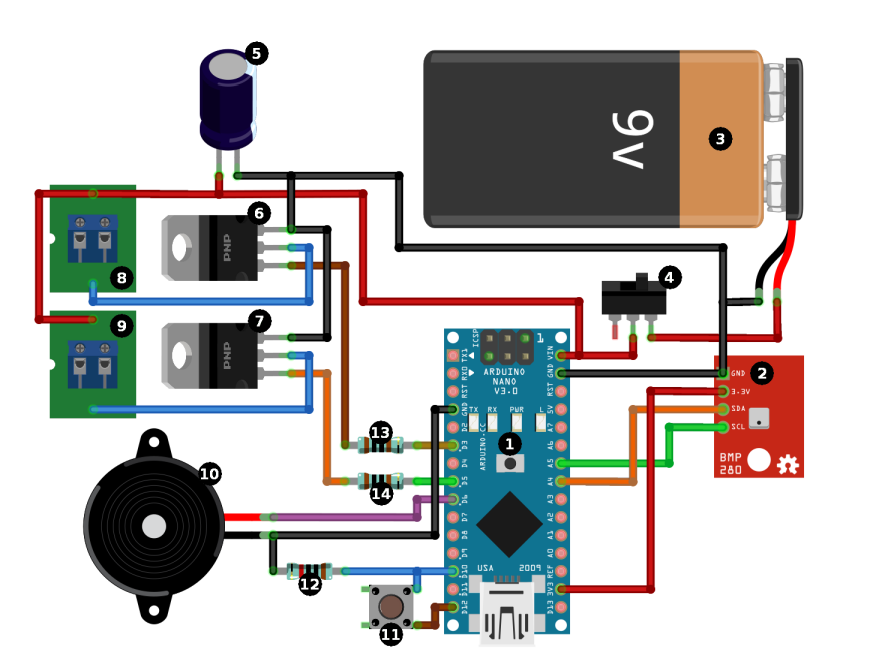
\includegraphics[width=0.6\textwidth]{./fig/electronics}
\caption{Ilustração do esquema elétrico do rRocket}.
\label{fig:rRocketelectronics}
\end{figure}

Ignitores elétricos podem utilizar mais corrente do que a baterias 6LR61 conseguem fornecer. Além disso, o aumento da corrente elétrica faz com que a tensão nos terminais da bateria diminua. Para uma corrente suficientemente alta, é possível que a tensão seja tão baixa a ponto de desligar o Arduino. Para contornar esse problema, o rRocket utiliza uma capacitor para armazenar energia elétrica e realizar o acionamento dos ignitores. Em testes de bancada, observou-se que capacitores eletrolíticos de 1000~$\mu$F carregados até ??~V são capazes de acionar ignitores com resistência de 1,6~$\Omega$ (Fig.~??). (\textbf{completar as informações}) Para carregar o capacitor sem sobrecarregar a bateria, utiliza-se um resistor como limitador de corrente. A escolha da resistência é descrita a seguir.
 
 Os autores não encontraram na literatura uma indicação padronizada de faixas de corrente que as baterias 6LR61 suportam. Os \textit{datasheets} normalmente apresentam gráficos de tensão da bateria \textit{versus} o tempo para diversas cargas resistivas. Tipicamente a resistência de 270~$\Omega$ é utilizada para indicar alto consumo (33~mA), embora a bateria possa fornecer correntes mais altas (250~mA) por um tempo menor. Com base nestas informações, considera-se razoável que a bateria forneça corrente constante de 33~mA e 50~mA em alguns momentos de pico de uso. 
 
A bateria deve alimentar diretamente o Arduino e o capacitor. 
De acordo com o site do fabricante\footnote{\url{https://store.arduino.cc/products/arduino-nano}}, o Arduino Nano consome cerca de 19~mA. Assumindo  uma corrente de pico de 50~mA na bateria, o resistor do capacitor foi dimensionado em 330~$\Omega$, o que leva ao consumo de pico para carga do capacitor seja de 27~mA (9~V/330~$\Omega$). 


O resistor de base dos transístores TIP122 foi dimensionado em 470~$\Omega$ para que a corrente no pino digital do Arduino seja da ordem de 10~mA. \textbf{Concluir a elaboração}.


\textbf{Inserir foto do rRocket2022 e do rRocket-EZ montados}.

\section{\textit{Software}}
\label{sec:software}

%\subsection{Projeto de \textit{software}}

A estrutura do código-fonte do rRocket foi elaborada para refletir a estrutura do seu \textit{hardware} e levar em conta a trajetória esperada para voos típicos de minifoguetes, bem como as situações adversas da Seç.~\ref{sec:adversities}.

A representação do \textit{hardware} no código-fonte foi baseada no paradigma de Orientação a Objetos e implementada na linguagem C++. O dispositivo é representado através da classe \textit{RecoverySystem}, que por sua vez, contém instâncias das classes \textit{Barometer}, \textit{Actuator}, \textit{Memory}, \textit{Button} e \textit{HumanInterface}. A Fig.~\ref{fig:uml} apresenta um diagrama UML das classes do rRocket e seus métodos públicos.
Cada classe possui tarefas bem definidas:
\begin{itemize}
	\item \textit{RecoverySystem}: responsável pela gestão do sistema de recuperação;
	\item \textit{Barometer}: responsável pela leitura do sensor BMP280, registro da altura atual e do apogeu;
	\item \textit{Actuator}: responsável pela implantação do paraquedas auxiliar (\textit{drogue}) e do paraquedas principal;
	\item \textit{Memory}: responsável pela gestão da memória EEPROM (gravação e leitura de dados);
	\item \textit{Button}: responsável pela observação do estado do botão. O botão pode estar em um dos seguintes estados: solto (\textit{released}), pressionado (\textit{pressed}), pressionado e solto em seguida (\textit{pressedAndReleased}) e pressionado longamente (\textit{longPressed}).
	\item \textit{HumanInterface}: responsável pela comunicação com o usuário através da porta serial (USB), LED (visual) e \textit{buzzer} (sonoro).
\end{itemize}

\begin{figure}[!ht]
	\centering
	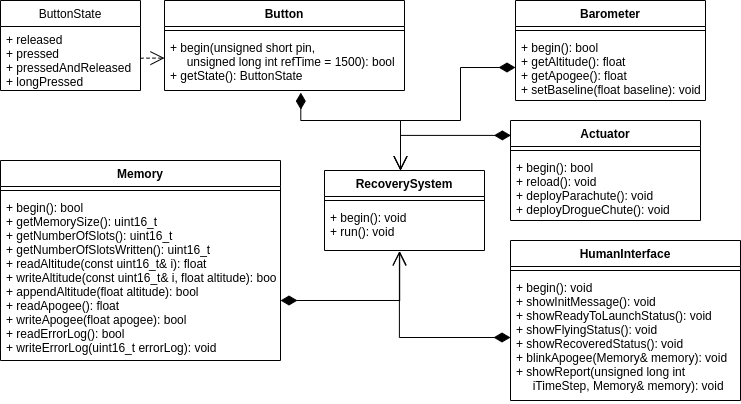
\includegraphics[width=0.99\textwidth]{./fig/RecoverySystem}
	\caption{Diagrama UML das classes do rRocket.}
	\label{fig:uml}
\end{figure}

Para realizar a gestão do sistema de recuperação, a classe \textit{RecoverySystem} utiliza o conceito de \textit{Máquina de Estados Finitos}. Neste conceito, o comportamento do dispositivo muda de acordo com o seu estado e o estado muda de acordo com eventos predeterminados. 

Considerando a trajetória típica de voo de minifoguetes (Fig.~\ref{fig:trajectoryA}), foram identificados cinco estados para o dispositivo:
\begin{itemize}
	\item \textit{readyToFly} (A$\to$ B): o dispositivo está aguardando o lançamento;
	\item \textit{flying} (B$\to$ E): o dispositivo está em voo;
	\item \textit{drogueChuteActive} (E$\to$ F): o dispositivo está em queda com a implantação do paraquedas auxiliar;
	\item \textit{parachuteActive} (F$\to$ G): o dispositivo está em queda com a implantação do paraquedas principal;
	\item \textit{recovered} (G$\to$ H): o dispositivo foi recuperado.
\end{itemize} 

A Figura~\ref{fig:states} apresenta nos balões os estados possíveis para o sistema de recuperação. As setas entre os balões indicam os eventos que geram as mudanças de estado e o sentido da mudança.
\begin{figure}[!ht]
	\centering
	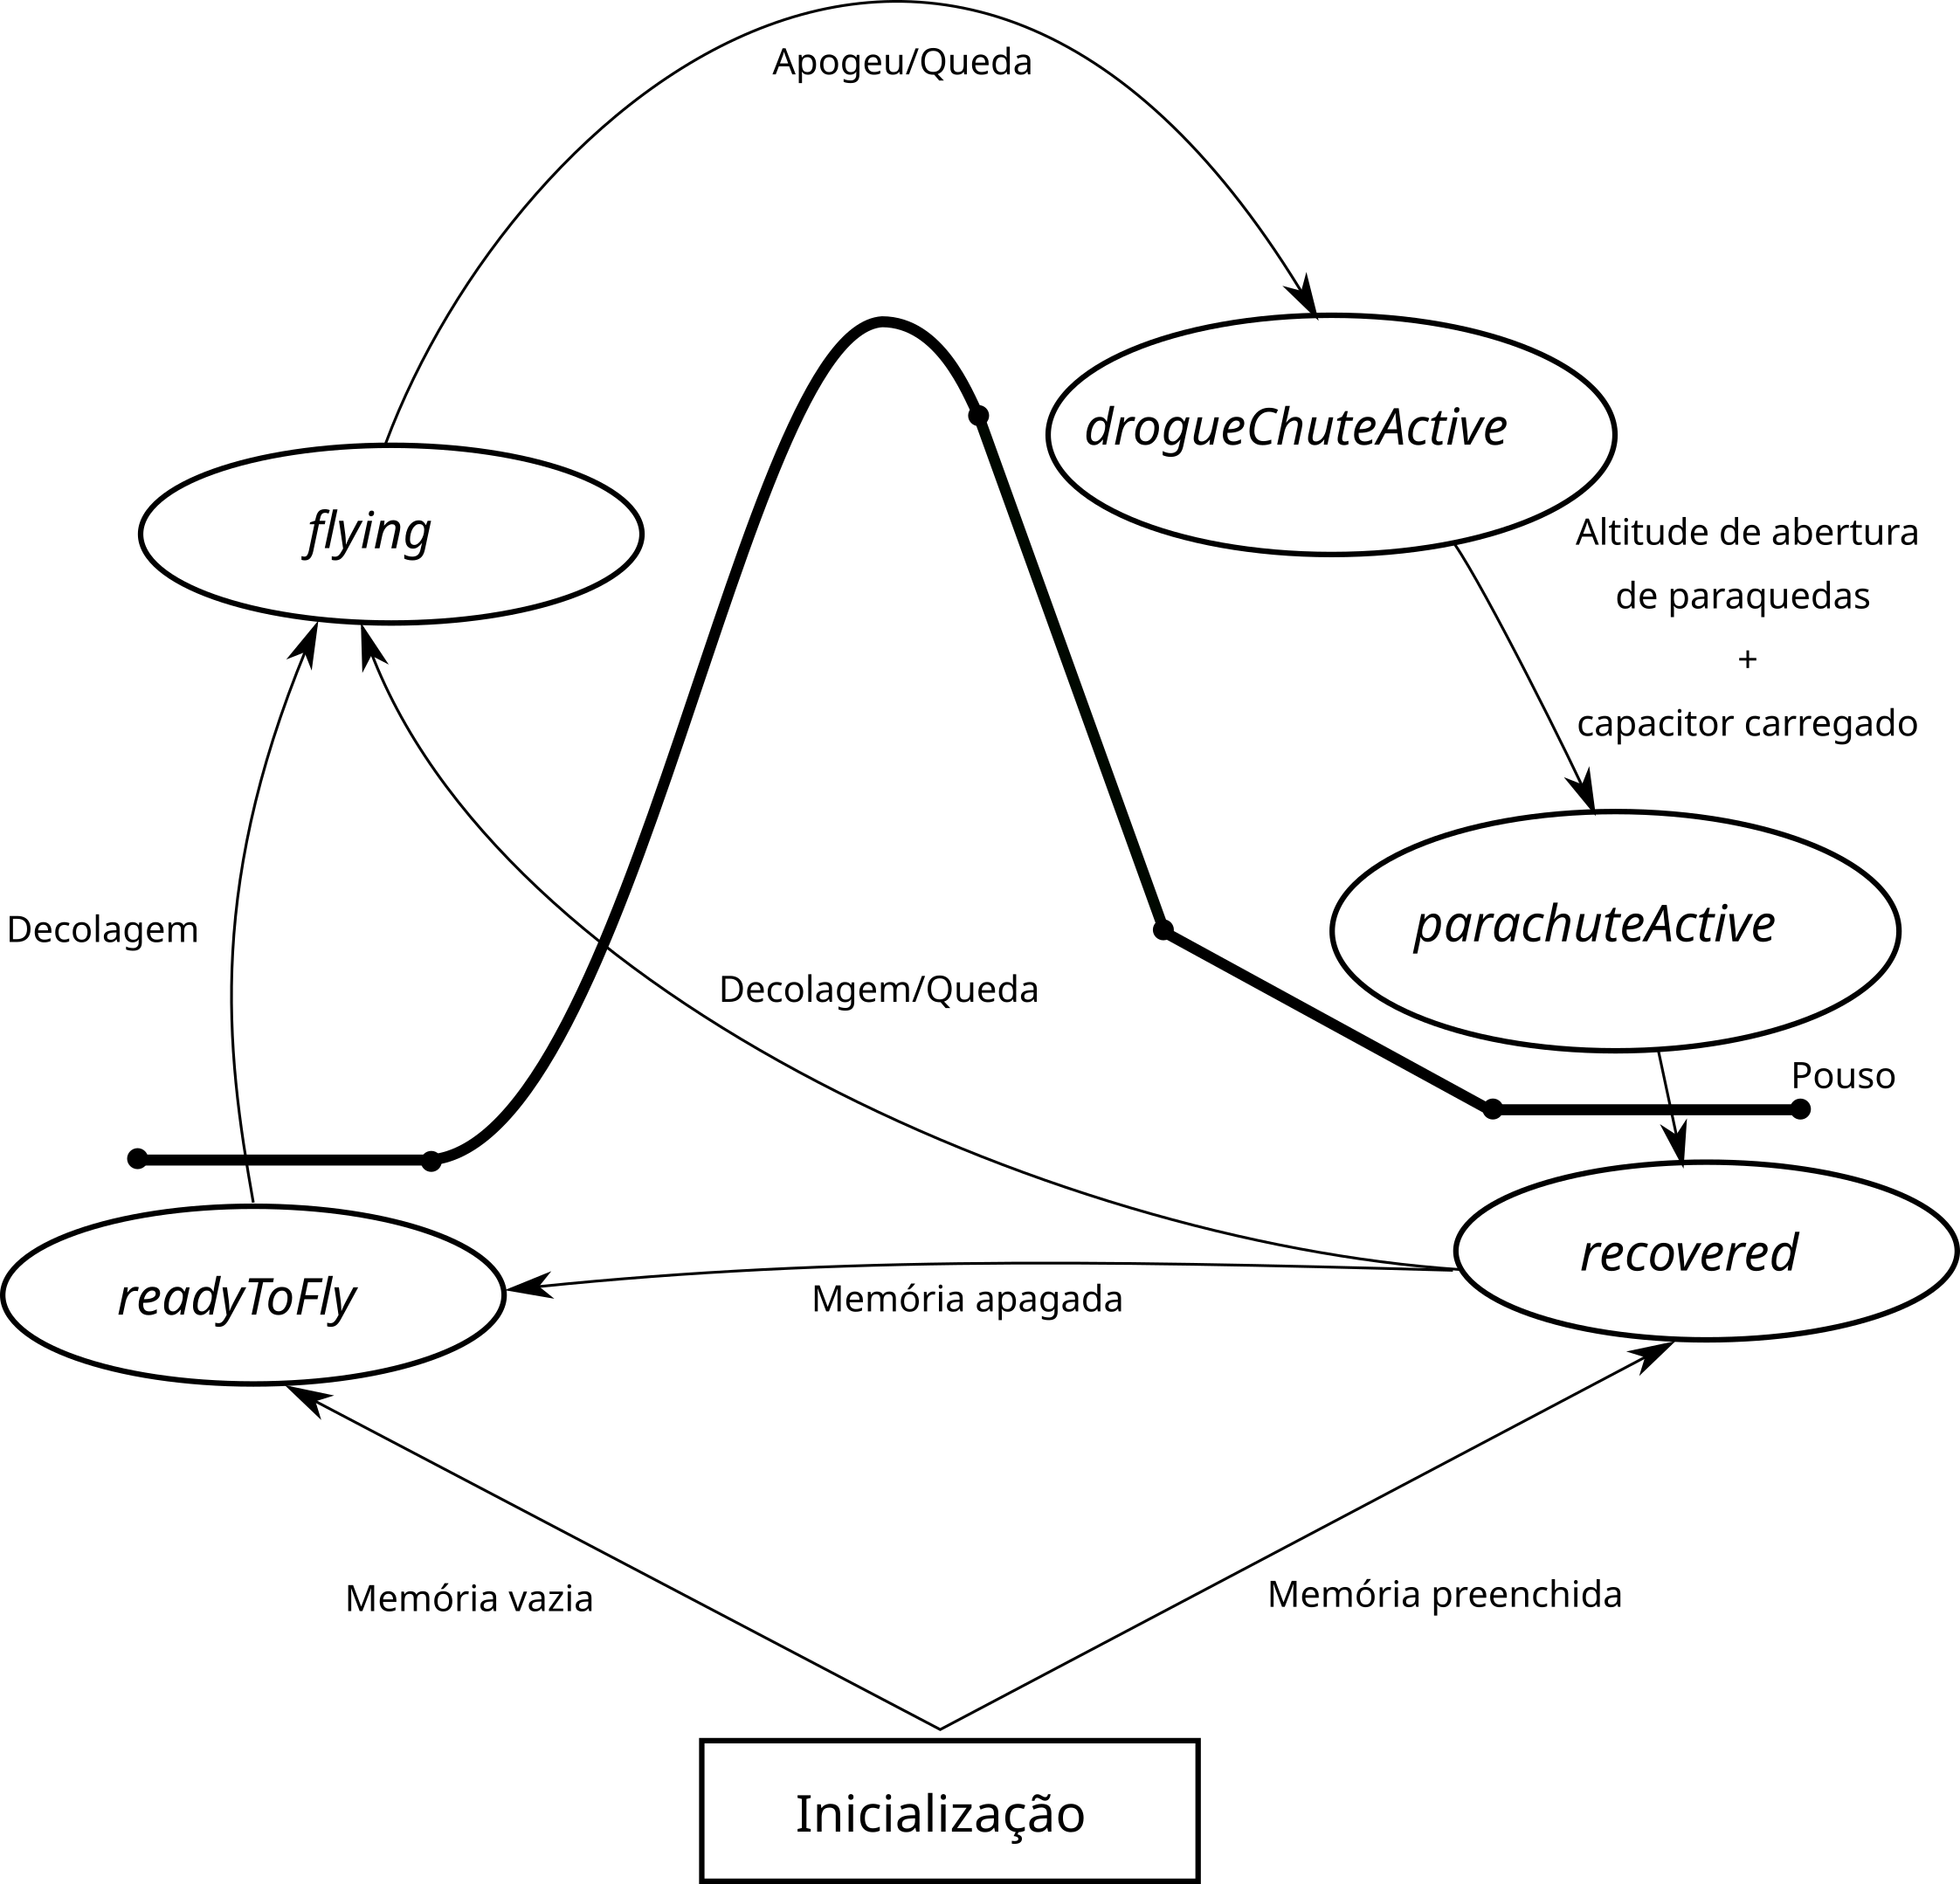
\includegraphics[width=0.8\textwidth]{./fig/FSM}
	\caption{Diagrama de estados e eventos do rRocket.}
	\label{fig:states}
\end{figure}

Existem cinco eventos que geram mudanças de estado:
\begin{itemize}
	\item Decolagem: o critério de decolagem da Seç.~\ref{sec:flightevents} foi satisfeito.
	\item Queda: o critério de queda da Seç.~\ref{sec:flightevents} foi satisfeito.
	\item Altitude de abertura de paraquedas + capacitor carregado: o critério de implantação de paraquedas principal da Seç.~\ref{sec:flightevents} foi satisfeito e o capacitor para acionamento dos ignitores elétricos está carregado.
	\item Pouso: o critério de pouso da Seç.~\ref{sec:flightevents} foi satisfeito.
	\item Memória apagada: o usuário requisitou a limpeza da memória para o próximo voo.
\end{itemize}

Note na Figura~\ref{fig:states} que o estado inicial do altímetro depende do estado da memória. Se já houver dados gravados, o altímetro inicia no estado \textit{recovered}. Nesse estado, o altímetro fica sensível à decolagem ou à queda. Isso é necessário para lidar com reinicialização do altímetro durante o voo (situação adversa 8 - Seç.~\ref{sec:adversities}). \textbf{É fundamental que o usuário limpe a memória antes de cada voo.} Se o altímetro for lançado no estado \textit{recovered}, o critério de queda pode ser satisfeito imediatamente após o lançamento, devido à situação adversa 5 (Seç.~\ref{sec:adversities}), causando a implantação prematura dos paraquedas. Caso a memória esteja limpa na inicialização, ou ainda, caso a memória seja apagada enquanto o estado é \textit{recovered}, o estado do altímetro é alterado para \textit{readyToFly}. Este estado é sensível apenas ao evento de decolagem, para evitar a situação adversa 5.

Caso o altímetro detecte decolagem no estado \textit{readyToFly} ou caso detecte decolagem OU queda no estado \textit{recovered}, o estado do altímetro é alterado para \textit{flying}. Os dados do vetor $h_k$ são gravados na memória permanente (EEPROM). Durante o voo, no estado \textit{flying}, as condições de apogeu e queda são monitoradas. Se qualquer uma delas for satisfeita, o estado do altímetro é alterado para \textit{drogueChuteActive}. Neste estado, o atuador inicia o primeiro ciclo de disparo do paraquedas auxiliar. O ciclo consiste em manter o ignitor elétrico ligado pelo intervalo de tempo $T_\text{act}$ e desligado pelo intervalo de tempo $T_\text{recharge}$, para permitir que o capacitor seja recarregado. O usuário pode definir quantas vezes o ciclo deve ser repetido $N_\text{attempt}$. A redundância nos disparos é uma forma de mitigar a situação adversa 11. Caso a altitude de lançamento do paraquedas principal seja alcançada e o ciclo de disparo do paraquedas auxiliar tenha sido concluído, o estado do altímetro é alterado para \textit{parachuteActive}. Note que não é necessário que todas as tentativas de disparo do paraquedas auxiliar tenham sido executadas para a mudança de estado. Basta que um dos ciclos de disparo tenha sido concluído. No estado \textit{parachuteActive}, o atuador inicia o ciclo de disparo do paraquedas principal. O ciclo é repetido até $N_\text{attempt}$ vezes. Caso o critério de pouso seja satisfeito, o estado do altímetro é alterado para \textit{recovered}. Neste estado, o altímetro não registra mais os dados de voo na memória e observa o estado do botão. Se o botão for pressionado por menos de 3 segundos, o \textit{buzzer}, o \textit{LED} e a comunicação serial são utilizados para informar os dados do último voo. Caso pressionado por mais de 3 segundos, a memória é apagada.

No estado \textit{readyToFly}, o altímetro liga o LED e aciona o \textit{buzzer} a cada 1,5 segundos para indicar que o sistema está pronto para o lançamento. O usuário não deve lançar o minifoguete se esta condição não for satisfeita.

No estado \textit{recovered}, ao pressionar o botão por menos de 3 segundos, o altímetro apresenta o relatório do último voo. O apogeu é apresentado através de acionamentos rápidos do LED e do \textit{buzzer}. Cada piscada/\textit{beep} curta corresponde a uma unidade. Uma piscada/\textit{beep} longa indica o algarismo 0. O altímetro indica inicialmente a casa dos milhares (se necessário). Em seguida indica a casa das centenas (se necessário) e assim por diante. Cada casa decimal é separada por uma breve pausa. Após a apresentação do apogeu, os dados de tempo e altitude são enviados através da comunicação serial.

Todos os parâmetros de configuração estão em um único arquivo arquivo \textit{Parameters.h}. Na Tab.~\ref{tab:parameters} estão listados os parâmetros e seus significados.

\begin{table}[!ht]
	\centering
\caption{Parâmetros de configuração do rRocket}
	\small
\begin{tabular}{r|p{1.5cm}|p{9cm}}
\hline
\hline
Variável&Valor&Significado\\
\hline
\textit{softwareVersion}&rRocket v.1.5.6& Versão do \textit{firmware}\\
\textit{pinLed}&13 &Número do pino para o LED\\
\textit{pinBuzzer}&11& Número do pino para o \textit{buzzer}\\
\textit{pinButton}&10&Número do pino para o botão\\
\textit{pinDrogueChute}&12&Número do pino para o paraquedas auxiliar\\
\textit{pinParachute}&3&Número do pino para o paraquedas principal\\
\textit{speedForLiftoffDetection}&30&Velocidade para detectar lançamento ($\bar{v}_\text{liftoff}$) - m/s\\
\textit{speedForFallDetection}&30&Velocidade para detectar queda ($\bar{v}_\text{fall}$) - m/s\\
\textit{speedForApogeeDetection}&7&Velocidade para detectar apogeu ($\bar{v}_\text{apogee}$) - m/s\\
\textit{parachuteDeploymentAltitude}&200&Altura para disparar o paraquedas principal ($H_\text{parachute}$) - m\\
\textit{displacementForLandingDetection}&3&Deslocamento para detectar pouso ($D_\text{land}$) - m\\
\textit{maxNumberOfDeploymentAttempts}&3&Número máximo de tentativas de acionamento dos ignitores elétricos ($N_\text{attempt}$)\\
\textit{actuatorDischargeTime}&500&Tempo para manter o atuador ligado ($T_\text{act}$) - ms\\
\textit{capacitorRechargeTime}&1000&Tempo para manter o atuador desligado e recarregar o capacitor ($T_\text{recharge}$) - ms\\
\hline
\hline
\end{tabular}
\label{tab:parameters}
\end{table}

O altímetro também registra possíveis erros. A Tab.~\ref{tab:erros} lista os códigos de erro e seus significados.
\begin{table}[!ht]
	\caption{Códigos de erro do rRocket}
	\small
	\centering
	\begin{tabular}{c|p{8cm}}
		\hline
		\hline
		Código&Significado\\
		\hline
		0& Nenhum erro detectado\\
		1& Falha de inicialização do barômetro\\
		2& Falha de inicialização do atuador\\
		3& Altitude menor que o valor armazenável (16 bits)\\
		4& Altitude maior que o valor armazanável (16 bits)\\
		5& Voo iniciado com memória não vazia\\
		\hline
		\hline
	\end{tabular}
	\label{tab:erros}
\end{table}

\section{Testes}

Diversos testes foram planejados para avaliar os critérios de detecção de eventos de voo, o \textit{software} de controle e o \textit{hardware} do altímetro. Tais testes estão organizados em cinco categorias:
\begin{itemize}
	\item  
	A primeira visa avaliar os critérios de detecção de eventos de voo com base em trajetórias fabricadas e que levam em conta as adversidades mencionadas na Seç.~\ref{sec:adversities}. 
	\item A segunda categoria visa avaliar os critérios de detecção de eventos de voo com base em trajetórias de voos reais, cujos dados foram obtidos com altímetros comerciais. Cabe destacar que o altímetro rRocket não foi utilizado nas duas primeiras categorias. Elas servem apenas ao propósito de testar os critérios de detecção de eventos de voo. 
	\item A terceira categoria consiste em testes em bancada utilizando o altímetro no modo \textit{debug}. Neste modo, o barômetro não lê a pressão, mas utiliza algumas das trajetórias fabricadas da categoria anterior. Além disso, o altímetro imprime na porta serial o seu \textit{status} (tempo, altitude, velocidade e estado). O objetivo desta categoria é avaliar o funcionamento do algoritmo para alguns dos casos da primeira categoria de testes e também avaliar a capacidade de acionamento dos ignitores elétricos. As atividades dos terminais do paraquedas auxiliar, do paraquedas principal e do capacitor são monitoradas. 
	\item Na quarta categoria, o altímetro, em modo normal, é submetido a variações de pressão controladas. As atividades dos terminais do paraquedas auxiliar, do paraquedas principal e do capacitor são monitoradas. 
	\item A quinta categoria consiste em voos reais com o uso do rRocket.
\end{itemize}
\subsection{Critérios de detecção de eventos de voo - voos fabricados}
\label{sec:manufacturedflights}

Três funções são introduzidas para testar os critérios de detecção de eventos de voo: (i) $h_\text{base}(t)$, que modela uma trajetória com propulsão seguida de voo balístico, (ii) $h_{noise}(t)$ para adicionar o ruído com amplitude $U_h$ e (iii) $h_\text{pert}(t)$, que representa perturbações nas medições de pressão.

A função base $h_\text{base}(t)$ é definida como
\begin{equation}
h_\text{base}(t)=
\begin{cases}
0 & \text{se } t < t_B, \\
a_\text{prop}(t-t_B)^2/2 & \text{se } t_B\le t \le t_C, \\
h_C+v_{C}(t-t_C)-g(t-t_C)^2/2 & \text{se } t_C < t \le t_G, \\
h_G & \text{se } t_G < t,
\end{cases}
\end{equation}
onde $t_B$ é o instante de início da queima do propelente, $t_C=t_B+T_\text{burn}$, onde $T_\text{burn}$ é o tempo de queima do propelente, $a_\text{prop}$ é a aceleração constante durante a fase propulsada,  $h_G$ é a altitude de pouso do minifoguete. Os demais parâmetros são calculados como
\begin{equation}
h_C=a_\text{prop}(t_C-t_B)^2/2,
\end{equation} 
\begin{equation}
v_C=a_\text{prop}(t_C-t_B),
\end{equation} 
e
\begin{equation}
t_G=t_C+\frac{v_C+\sqrt{v_C^2+2g(h_C-h_G)}}{g}.
\end{equation}
O apogeu ocorre no instante $t_D$, dado por
\begin{equation}
t_D=t_C+\frac{v_C}{g}.
\end{equation}

O ruído $h_{noise}(t)$ é calculado como
\begin{equation}
h_{noise}(t)=U_h\cdot(2\mathcal{R}-1),
\end{equation}
onde $\mathcal{R}$ é uma variável aleatória com distribuição uniforme entre 0 e 1.

Por fim, a função de perturbação $h_{pert}(t)$ é dada por
\begin{equation}
h_\text{pert}(t)=h_\text{pert,1}(t)+h_\text{pert,2}(t)+h_\text{pert,3}(t),
\end{equation}
onde
\begin{equation}
h_\text{pert,i}(t)=
\begin{cases}
A\sin\left(2\pi\frac{t-t_{b,i}}{T_p}\right) & \text{se } t_{b,i} \le t \le t_{e,i}, \\
0 & \text{caso contrário.}
\end{cases},\quad 1\le i \le 3.
\end{equation}
$A$ representa a amplitude, $T_p$ o período, $t_{b,i}$ e $t_{e,i}$ os instantes de início e fim, respectivamente, da i-ésima perturbação.

A Tab.~\ref{tab:functiontestparameters} apresenta os valores padrão dos parâmetros das funções de teste. 
\begin{table}[!ht]
	\centering
	\caption{Parâmetros para as funções de teste.}
	\begin{tabular}{ccc}
		\toprule
		Parâmetro & Valor & Unidade\\
		\midrule
		$a_\text{prop}$&2g&m/s$^2$\\
		$T_\text{burn}$&3&s\\
		$t_B$&10&s\\
		$h_G$&40&m\\
		$U_h$&1&m\\
		$A$&50&m\\
		$T_p$&1,2&s\\
		$t_{b,1}$&$t_B/3$&s\\
		$t_{e,1}$&$t_{b,1}+T_p$&s\\
		$t_{b,2}$&$t_B$&s\\
		$t_{e,2}$&$0,8~t_B$&s\\
		$t_{b,3}$&$1,2t_{D}$&s\\
		$t_{e,3}$&$t_G$&s\\
		\bottomrule
	\end{tabular}
\label{tab:functiontestparameters}
\end{table}

Os parâmetros padrão para aplicação dos critérios de detecção de eventos de voo da Seç.~\ref{sec:flightevents} são dados na Tab.~\ref{tab:flightparameters}.
\begin{table}[!ht]
	\centering
	\caption{Parâmetros para os critérios de detecção de eventos de voo.}
	\begin{tabular}{ccc}
		\toprule
		Parâmetro & Valor & Unidade\\
		\midrule
		$N$&12&-\\
		$T$&0,25&s\\
		$v_\text{liftoff}$&30&m/s\\
		$v_\text{fall}$&30&m/s\\
		$v_\text{apogee}$&7&m/s\\
		$H_\text{parachute}$&200&m\\
		$D_\text{land}$&3&m\\
		\bottomrule
	\end{tabular}
	\label{tab:flightparameters}
\end{table}

Para avaliar os critérios de detecção de eventos de voo, 14 voos fabricados foram considerados. Os objetivos de cada caso são discutidos a seguir. O resumo das configurações de cada caso são dados na Tab.~\ref{tab:flightcases}.
\begin{itemize}
	\item \textbf{Caso 1}: $h(t)=h_\text{base}$ a trajetória é uma função suave, como se pode observar na Fig.~\ref{fig:case01}. A mesma figura apresenta os pontos onde os critérios de detecção de eventos foram satisfeitos e a velocidade calculada com o processo de suavização.  Observe que a localização dos pontos é condizente com o que se espera, exceto pelo atraso na detecção do apogeu. O atraso é causado pelo procedimento de suavização da velocidade e pode ser reduzido aumentando-se o parâmetro $v_\text{apogee}$. Note, no entanto, que a diferença entre o apogeu detectado (259,7~m) e o real (264,6~m) é de apenas 4,9~m. O atraso causado pela suavização é compensado pelas vantagens obtidas nos casos a seguir. 
	\item \textbf{Caso 2}: adiciona-se ruído à trajetória base, isto é, $h(t)=h_\text{base}+h_\text{noise}$. Como se pode observar na Fig.~\ref{fig:case02}, os critérios de detecção de eventos de voo continuam funcionando adequadamente.
	\item \textbf{Caso 3}: adiciona-se ruído e perturbações à trajetória base, $h(t)=h_\text{base}+h_\text{noise}+h_\text{pert}$ (Fig.~\ref{fig:case03}). Há três perturbações: (i) uma durante o período de espera para lançamento, simulando rajadas laterais de vento ou variações de pressão durante a montagem do minifoguete, (ii) uma logo após o lançamento, simulando uma trajetória instável e (iii) uma após o apogeu, simulando uma queda instável. Observe que a suavização da velocidade foi fundamental para a aplicação adequada dos critérios de detecção de eventos de voo.
	\item \textbf{Caso 4}: semelhante ao Caso 3, exceto pela perturbação em $h$ ser mantida ao longo de todo o voo. Os critérios de detecção de eventos de voo produzem resultados condizentes com o esperado (Fig.~\ref{fig:case04}).
	\item \textbf{Caso 5}: semelhante ao Caso 3, exceto pela aceleração de propulsão ser de apenas $g$, simulando assim, um minifoguete com baixa velocidade de lançamento. Note na Fig.~\ref{fig:case05} que o critério de implantação de paraquedas principal ocorre logo após o critério de detecção de apogeu, uma vez que o apogeu foi menor que os 200~m estipulados para o lançamento do paraquedas principal. Os demais critérios de detecção de eventos de voo produzem resultados condizentes com o esperado.
	\item \textbf{Caso 6}: semelhante ao Caso 3, exceto pela aceleração de propulsão ser de $6g$, simulando assim, um minifoguete com alta velocidade de lançamento.  Os critérios de detecção de eventos de voo produzem resultados condizentes com o esperado (Fig.~\ref{fig:case06}).
	\item \textbf{Caso 7}: semelhante ao Caso 3, exceto pela altitude de pouso ser menor que a de lançamento. Este caso, assim como o 3, serve para avaliar a situação adversa 7, da Seç.~\ref{sec:adversities}.  Os critérios de detecção de eventos de voo produzem resultados condizentes com o esperado (Fig.~\ref{fig:case07}).
	\item \textbf{Caso 8}: semelhante ao Caso 3, exceto pelo período da perturbação ser metade do original ($T_p=0,6$~s). Os critérios de detecção de eventos de voo produzem resultados condizentes com o esperado (Fig.~\ref{fig:case08}).
	\item \textbf{Caso 9}: semelhante aos Casos 3 e 8, exceto pelo período da perturbação ser o dobro do original ($T_p=2,4$~s). Os critérios de detecção de eventos de voo \textbf{falham} na primeira perturbação (Fig.~\ref{fig:case09}). Dos Casos 3, 8, 9, 10 e 11, observa-se que o procedimento de suavização é mais efetivo quando ao período utilizado no cálculo das médias ($\tau=NT/2=1,5$~s) é maior que o período da perturbação $T_p$, \textit{i.e}, $\tau>T_p$. Aumentar $\tau$, no entanto, gera atraso na detecção de eventos. Os voos reais, analisados na próxima seção, apresentaram perturbações com períodos de oscilação menor ou igual a 0,8~s.
	\item \textbf{Caso 10}: semelhante ao Casos 3, exceto pelo número de períodos de observação ($N=8$). Os critérios de detecção de eventos de voo \textbf{falham} na primeira perturbação (Fig.~\ref{fig:case10}), pois, como comentado no item anterior, houve redução de $\tau$. 
	\item \textbf{Caso 11}: semelhante ao Casos 3, exceto pelo número de períodos de observação ($N=16$). Os critérios de detecção de eventos de voo produzem resultados condizentes com o esperado (Fig.~\ref{fig:case11}). Houve, como esperado, um atraso maior na detecção do apogeu.
	\item \textbf{Caso 12}: semelhante ao Casos 3, exceto pelo número de períodos de observação ($N=24$) e período de leitura da pressão ($T=0,125$~s). Os critérios de detecção de eventos de voo produzem resultados condizentes com o esperado e semelhantes ao do Caso 3, exceto por uma resolução maior na trajetória (Fig.~\ref{fig:case12}).
	\item \textbf{Caso 13}: semelhante ao Casos 3, exceto pela aceleração de propulsão ($3g$) e início de leitura dos dados, simulando uma reinicialização do altímetro antes do apogeu. Os critérios de detecção de eventos de voo produzem resultados condizentes com o esperado (Fig.~\ref{fig:case13}).
	\item \textbf{Caso 14}: semelhante ao Casos 3, exceto pela aceleração de propulsão ($3g$) e início de leitura dos dados, simulando uma reinicialização do altímetro após o apogeu. Os critérios de detecção de eventos de voo produzem resultados condizentes com o esperado (Fig.~\ref{fig:case14}).
\end{itemize}
\begin{table}[!ht]
	\centering
	\caption{Configurações dos casos avaliados.}
	\begin{tabular}{ccc}
		\toprule
		Caso & Função $h(t)$ & Parâmetros\\
		\midrule
		1&$h_\text{base}$& Padrão\\
		2&$h_\text{base}+h_\text{noise}$& Padrão\\
		3&$h_\text{base}+h_\text{noise}+h_\text{pert}$& Padrão\\
		4&$h_\text{base}+h_\text{noise}+h_\text{pert}$& Padrão, exceto $t_{e,2}=1,2t_D$\\
		5&$h_\text{base}+h_\text{noise}+h_\text{pert}$& Padrão, exceto $a_\text{prop}=g$\\
		6&$h_\text{base}+h_\text{noise}+h_\text{pert}$& Padrão, exceto $a_\text{prop}=6g$\\
		7&$h_\text{base}+h_\text{noise}+h_\text{pert}$& Padrão, exceto $h_G=-40~\text{m}$\\
		8&$h_\text{base}+h_\text{noise}+h_\text{pert}$& Padrão, exceto $T_p=0,6~\text{s}$\\
		9&$h_\text{base}+h_\text{noise}+h_\text{pert}$& Padrão, exceto $T_p=2,4~\text{s}$\\		
		10&$h_\text{base}+h_\text{noise}+h_\text{pert}$& Padrão, exceto $N=8$\\	
		11&$h_\text{base}+h_\text{noise}+h_\text{pert}$& Padrão, exceto $N=16$\\	
		12&$h_\text{base}+h_\text{noise}+h_\text{pert}$& Padrão, exceto $N=24$ e $T=0,125$~s \\	
		13&$h_\text{base}+h_\text{noise}+h_\text{pert}$& Padrão, reinicialização em voo ($a_\text{prop}=3g$, $t>0,5(t_B+t_D)+t_B$) \\
		14&$h_\text{base}+h_\text{noise}+h_\text{pert}$& Padrão, reinicialização em voo ($a_\text{prop}=3g$, $t>t_D$) \\
		\bottomrule
	\end{tabular}
	\label{tab:flightcases}
\end{table}

\subsection{Critérios de detecção de eventos de voo - voos reais}
\label{sec:realflightsforeventsverification}

Sete voos reais foram utilizados para testar os critérios de detecção de eventos de voo. Os voos são representativos de situações típicas de lançamentos:
\begin{itemize}
	\item Lançamento 1: voo bem-sucedido com apogeu entre 200 e 500 m e com baixa velocidade de saída da rampa. Identificação: Netuno-F/Paraná-25/v2, LT 2 Dez 2019, apogeu = 285 m.
	
	\item Lançamento 2: voo bem-sucedido com apogeu entre 500 e 1000 m e com alta velocidade de saída da rampa. Identificação: Netuno-R-B/Paraná-7b, LT 7 Set 2017, apogeu = 794 m.
	
	\item Lançamento 3: voo bem-sucedido com apogeu acima de 1000 m e velocidade próxima à do som (Mach 0.9). Identificação: Urano/Paraná-15b, LT 7 Set 2018, apogeu = 1216 m.
	
	\item Lançamento 4: voo bem-sucedido com velocidade típica de saída da rampa. Identificação: Netuno-R-B/Paraná-26/v2, LT 2 Dez 2019, apogeu = 541 m.
	
	\item Lançamento 5: voo instável com rotação na direção vertical. Amplitude e frequência das oscilações: 125 m e 0,2~s. Identificação: Netuno-R-B/Paraná-7, LT 24 Jun 2017, apogeu = 271 m.
	
	\item Lançamento 6: voo instável lateral. Amplitude e frequência das oscilações: 85 m e 0,74~s. Identificação: 
	Urano/Paraná-30, LT 9 Jan 2022, apogeu = 58 m.
	
	\item Lançamento 7: voo instável lateral.  Amplitude e frequência das oscilações: 15 m e 0,8~s. Identificação:
	Plug/Paraná-24/v2, LT 15 Nov 2019, apogeu (visual) = 40 a 60 m.
\end{itemize}

Os gráficos das trajetórias e os pontos que representam os eventos de voo (considerando os parâmetros da Tab.~\ref{tab:flightparameters}) são apresentados nas Figs.~\ref{fig:lancamento01}-\ref{fig:lancamento07-15}. Os critérios de detecção de eventos de voo produziram resultados coerentes em todos os voos, exceto pelo Lançamento 7. Neste último caso, o lançamento não foi detectado pois $\bar{v}_y<\bar{v}_\text{liftoff}=30$~m/s. O parâmetro $\bar{v}_\text{liftoff}$ pode ser ajustado pelo usuário. Se $\bar{v}_\text{liftoff}=15$~m/s, por exemplo, então os eventos de voo são detectados, como se pode observar na Fig.~\ref{fig:lancamento07-15}. Cabe notar que o altímetro comercial StratoLogger também não detectou o Lançamento 07. Além disso, não é recomendável um valor muito baixo para $\bar{v}_\text{liftoff}$, pois se o altímetro estiver ligado durante a montagem do minifoguete, variações de pressão podem causar detectar lançamento falso e causar o acionamento prematuro dos paraquedas (situação adversa 6).

\subsection{Barômetro simulado}
\label{sec:simulations}
O objetivo deste conjunto de testes é avaliar o funcionamento do altímetro rRocket sob condições muito controladas. Para isso, o trecho de código responsável por retornar a leitura do barômetro real é substituída por um barômetro simulado, que retorna $h(t)$ de acordo com alguma trajetória fabricada.

Em todas as nove simulações monitorou-se o sinal elétrico nos terminais do capacitor e dos terminais dos paraquedas. Nas sete primeiras simulações, o altímetro ficou ligado à porta serial para que seu estado fosse monitorado. Para evitar problemas elétricos, nestas simulações o altímetro foi alimentado apenas através de cabo USB (a bateria 6LR61 não foi utilizada). Nas duas últimas simulações, a bateria foi ligada e o cabo USB desconectado do altímetro.

O resumo das simulações é apresentado na Tab.~\ref{tab:simulations}. As descrições completas das simulações e os resultados obtidos são apresentados a seguir:
\begin{itemize}
	\item Simulação 1: utiliza a trajetória do Caso 3 da Seç.~ \ref{sec:manufacturedflights} que representa um voo com perturbações e ruídos. O altímetro é inicializado com a memória vazia. Os resultados da simulação são apresentados na Fig.~\ref{fig:sim01}. O eixo vertical da esquerda apresenta a altitude. O eixo vertical da direita representa o sinal elétrico (proporcional à tensão) medido no capacitor e nos terminais dos paraquedas. A trajetória registrada na memória EEPROM coincide com a trajetória lida em tempo real através da comunicação serial. Além disso, o altímetro detectou corretamente os eventos de voo. As letras ao lado das curvas indicam o estado do altímetro: R = \textit{readyToFly}, F=\textit{flying}, D=\textit{drogueChuteActive}, P=\textit{parachuteActive} e L=\textit{recovered}. Note que a tensão no capacitor ficou praticamente constante ao longo de todo o voo. Isso ocorreu porque os terminais dos paraquedas ficaram abertos nesta simulação. Também é possível observar as três tentativas de acionamento do paraquedas auxiliar (\textit{drogue}) e do paraquedas principal.
	\item Simulação 2: semelhante à Simulação 1, exceto pelo fato da memória não ser apagada antes do voo. Note na Fig.~\ref{fig:sim02} que o altímetro é inicializado no estado \textit{recovered}, como esperado, e que a memória contém os dados do último voo. Embora o voo ocorra a partir do estado \textit{recovered}, o altímetro funciona corretamente, fazendo o acionamento dos paraquedas. O relatório de voo indica o erro 5, da tabela de erros, isto é ``Voo iniciado com memória não vazia".
	\item Simulação 3: semelhante Simulação 2, exceto pelo deslocamento do tempo em 16~s, simulando a reinicialização do altímetro em voo. Observe na Fig.~\ref{fig:sim03} que o paraquedas auxiliar é acionado apenas uma vez, pois a condição de abertura de paraquedas já está satisfeita no instante em que o paraquedas auxiliar seria acionado pela segunda vez. Neste caso, a prioridade é acionar o paraquedas e, portanto, o altímetro altera seu estado de \textit{drogueChuteActive} para \textit{parachuteActive}. Em seguida, o paraquedas é acionado três vezes. O altímetro se comporta como esperado. 
	\item Simulação 4: semelhante ao Caso 3, exceto por $a_\text{prop}=10g$, $T_\text{burn}=5$~s. O objetivo desta simulação é avaliar como a trajetória é registrada na memória quando o apogeu excede o limite superior (6000~m). Deve-se lembrar que, devido à restrição de memória EEPROM, decidiu-se armazenar a altitude como uma variável de 16 bits. Observe na Fig.~\ref{fig:sim04} que a trajetória armazenada na memória do altímetro foi modulada ao intervalo de -500 a 6000~m. Desta forma é possível que o usuário consiga recuperar os dados do voo. O altímetro operou corretamente.
	\item Simulação 5: semelhante ao Caso 3, exceto por $h_G=-1600$. Esta trajetória simula a situação em que a altitude final da trajetória é menor que o limite inferior (-500~m) para armazenamento na memória do altímetro. Como se pode observar na Fig.~\ref{fig:sim05}, a altitude registrada na memória EEPROM foi modulada para permanecer no intervalo -500 a 6000~m. O altímetro operou corretamente.
	\item Simulação 6: simula a trajetória do Caso 5, isto é, um voo com apogeu inferior a 100~m e com baixa velocidade de saída da rampa. Como se pode observar na Fig.~\ref{fig:sim06}, o altímetro funcionou como esperado.
	\item Simulação 7: simula a trajetória do Caso 6, isto é, um voo com apogeu de cerca de 1800~m e alta velocidade de lançamento. Como se pode observar na Fig.~\ref{fig:sim07}, o altímetro funcionou como esperado.
	\item Simulação 8: simula a trajetória do Caso 3. O objetivo é avaliar a capacidade do altímetro em acionar quatro ignitores elétricos (dois ligados em paralelo aos terminais do paraquedas auxiliar e outros dois em paralelo aos terminais do paraquedas principal). Cada ignitor tem resistência média de (1,6$\pm$0,1)~$\Omega$. Diferentemente da Simulação 1, nesta, o altímetro é alimentado por uma bateria 6LR61. No momento do teste, a tensão da bateria era de 8,54~V e a tensão no capacitor de 7,73~V. Como se pode observar na Fig.~\ref{fig:sim08}, há quedas de tensão abruptas (cerca de 1~ms) seguidas de recarga lenta (cerca de 1~s) no capacitor em todas as seis vezes em que os paraquedas são acionados, como esperado. Durante o acionamento do paraquedas auxiliar (\textit{drogue}) apenas um ignitor foi acionado na primeira tentativa. O outro resistor foi acionado na segunda tentativa. Isso reforça a importância das várias tentativas de acionamento. Já para o paraquedas principal, os dois ignitores foram acionados na primeira tentativa.
	
	\item Simulação 9: simula a trajetória do Caso 5. O objetivo é avaliar a capacidade do altímetro em acionar dois ignitores elétricos em sequência (um ligado aos terminais do paraquedas auxiliar e outro aos terminais do paraquedas principal). Como se pode observar na Fig.~\ref{fig:sim09}, há quatro quedas de tensão no capacitor, uma para acionamento do \textit{drogue} e três para acionamento do paraquedas principal. Os dois \textit{squibs} foram ignitados corretamente na primeira tentativa.
\end{itemize}

\begin{table}[!ht]
	\centering
	\caption{Resumo das simulações em bancada com o altímetro}
	\begin{tabular}{cccc}
		\toprule
		&&\multicolumn{2}{c}{Terminais}\\\cmidrule{3-4}
		Num.&Descrição&\textit{Drogue}&Paraquedas\\
		\midrule
		Sim. 1 & Caso 3 & aberto&  aberto\\
		Sim. 2 & Caso 3 + \textit{recovered} & aberto&  aberto\\
		Sim. 3 & Caso 3 + \textit{recovered}+$t\ge 16$~s& aberto&  aberto\\
		Sim. 4 & Caso 3, exceto ($a_\text{prop}=10g$, $T_\text{burn}=5$~s)& aberto&  aberto\\
		Sim. 5 & Caso 3, exceto ($h_G=-1600$)~m& aberto&  aberto\\
		Sim. 6 & Caso 5 &  aberto&  aberto\\
		Sim. 7 & Caso 6 &  aberto&  aberto\\
		\midrule
		Sim. 8 & Caso 3 & 2 \textit{squibs}&  2 \textit{squibs}\\
		Sim. 9 & Caso 5 & 1 \textit{squib}&  1 \textit{squib}\\
		\bottomrule
	\end{tabular}
	\label{tab:simulations}
\end{table}

\subsection{Testes em bancada}

Para avaliar o funcionamento do rRocket em modo normal de operação, produziu-se uma câmara (Fig.~\ref{fig:instrumentation}) onde é possível variar a pressão sob o altímetro. Esta câmara também é equipada com um barômetro e faz o monitoramento do sinal elétrico (proporcional à tensão) no capacitor e nos terminais dos paraquedas.
\begin{figure}[!ht]
	\centering
	\includegraphics[width=0.8\textwidth]{./fig/instumentation}
	\caption{Aparato para instrumentação do rRocket em testes de bancada.}
	\label{fig:instrumentation}
\end{figure}

Sete experimentos foram realizados para avaliar o comportamento do altímetro em situações adversas. O resumo dos experimentos encontra-se na Tab.~\ref{tab:experimentation} e os detalhes de cada um são apresentados a seguir:
\begin{itemize}
\item Experimento 1: a variação de pressão é ajustada para simular um voo suave. A memória do altímetro foi apagada antes do experimento, de tal modo que o seu estado inicial é \textit{readyToFly}. Na Fig.~\ref{fig:exp01} é possível observar que a trajetória registrada pela instrumentação da câmara coincide com a registrada pelo altímetro (EEPROM) (eixo vertical à esquerda). Além disso, é possível observar na figura o sinal elétrico no capacitor e nos terminais dos paraquedas (eixo vertical à direita). O altímetro operou corretamente.
\item Experimento 2: a variação de pressão é ajustada para simular um voo suave, porém, a memória do altímetro não foi apagada antes do experimento, de tal modo que o seu estado inicial é \textit{recovered}. Com se pode observar na Fig.~\ref{fig:exp02}, o altímetro operou corretamente. O relatório de voo registrou o código de erro 5, ou seja, ``Voo iniciado com memória não vazia", como esperado.
\item Experimento 3: a variação de pressão aplicada simula um voo instável. Há um decréscimo brusco em $h$ logo após o lançamento seguido de oscilações. Com se pode observar na Fig.~\ref{fig:exp03}, o altímetro operou corretamente.
\item Experimento 4: com a memória do altímetro parcialmente preenchida, de tal modo que seu estado inicial é \textit{recovered}, aplicou-se um aumento de pressão para simular uma reinicialização do altímetro em voo. Os resultados são apresentados na Fig.~\ref{fig:exp04}.  O altímetro detectou a queda e acionou os paraquedas.
\item Experimento 5: a pressão foi reduzida abruptamente para simular um voo com alta velocidade de lançamento. Os resultados são apresentados na Fig.~\ref{fig:exp05}. 
\item Experimento 6: a pressão foi variada de tal modo que o apogeu fosse menor que 200~m. O objetivo é avaliar o acionamento dos paraquedas. Note na Fig.~\ref{fig:exp06}, que o altímetro fez uma tentativa de acionamento do \textit{drogue} e, em seguida, fez três tentativas de acionamento do paraquedas, como esperado.
\item Experimento 7: a pressão foi controlada de modo a simular o Lançamento 3, onde se observa uma redução em $h$ imediatamente após a decolagem. Os dados do experimento são apresentados na Fig.~\ref{fig:exp07}. Mais uma vez, o altímetro se comportou corretamente.
\end{itemize}
\begin{table}[!ht]
	\centering
	\caption{Resumo dos experimentos em bancada com o altímetro}
	\begin{tabular}{cccc}
		\toprule
		&&\multicolumn{2}{c}{Terminais}\\\cmidrule{3-4}
		Num.&Descrição&\textit{Drogue}&Paraquedas\\
		\midrule
		Exp. 1 & Voo suave &  aberto&   aberto\\
		Exp. 2 & Voo suave + \textit{recovered} &  aberto&   aberto\\
		Exp. 3 & Voo instável &  aberto&   aberto\\
		Exp. 4 & Queda &   aberto& aberto\\
		Exp. 5 & Alta velocidade de lançamento&  aberto&   aberto\\
		Exp. 6 & Apogeu < 200~m&  aberto&   aberto\\
		Exp. 7 & Falsa queda na decolagem &  aberto&   aberto\\
		\bottomrule
	\end{tabular}
	\label{tab:experimentation}
\end{table}

\subsection{Testes em voo}

Descrever os testes em voos reais com o uso do rRocket.

\bibliography{/home/guilherme/Documentos/library/index}
\pagebreak
\newpage
\appendix

\section{Figuras}

\begin{figure}[!ht]
	\centering
	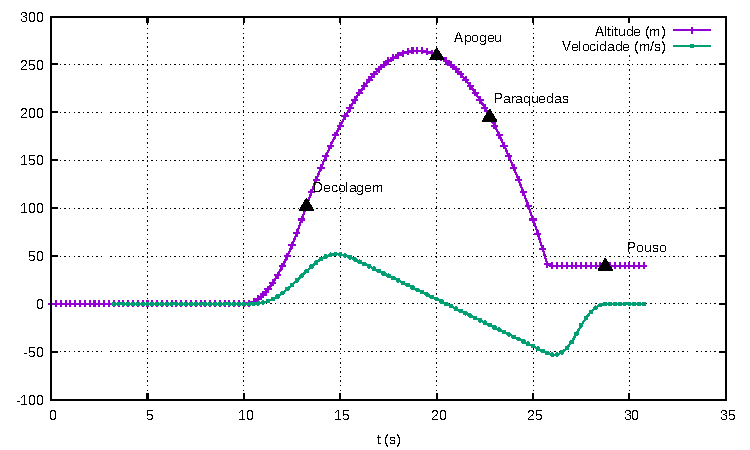
\includegraphics[width=\textwidth]{./data/cases/case01/trajectory}
	\caption{Aplicação dos critérios de detecção de eventos de voo. Caso 1}
	\label{fig:case01}
\end{figure}
\begin{figure}[!ht]
	\centering
	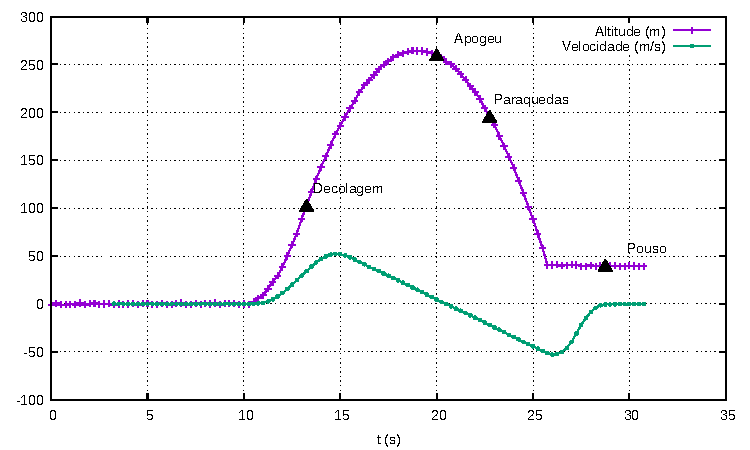
\includegraphics[width=\textwidth]{./data/cases/case02/trajectory}
	\caption{Aplicação dos critérios de detecção de eventos de voo. Caso 2}
	\label{fig:case02}
\end{figure}
\begin{figure}[!ht]
	\centering
	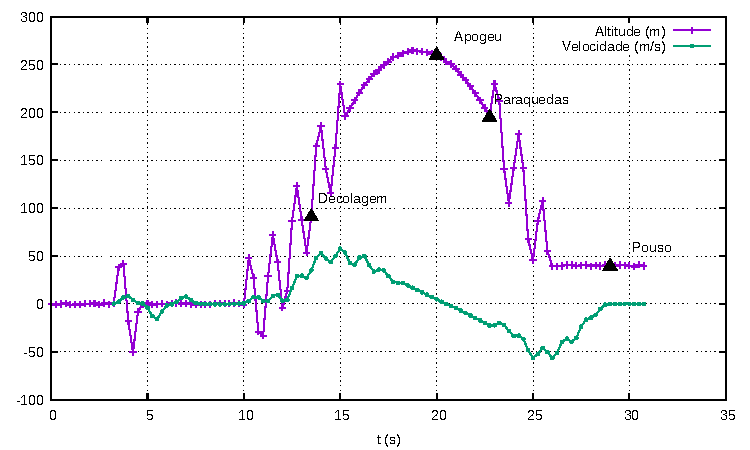
\includegraphics[width=\textwidth]{./data/cases/case03/trajectory}
	\caption{Aplicação dos critérios de detecção de eventos de voo. Caso 3}
	\label{fig:case03}
\end{figure}
\begin{figure}[!ht]
	\centering
	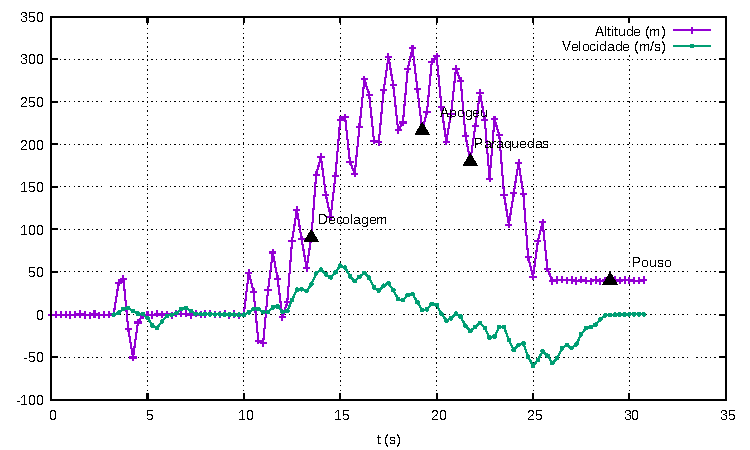
\includegraphics[width=\textwidth]{./data/cases/case04/trajectory}
	\caption{Aplicação dos critérios de detecção de eventos de voo. Caso 4}
	\label{fig:case04}
\end{figure}
\begin{figure}[!ht]
	\centering
	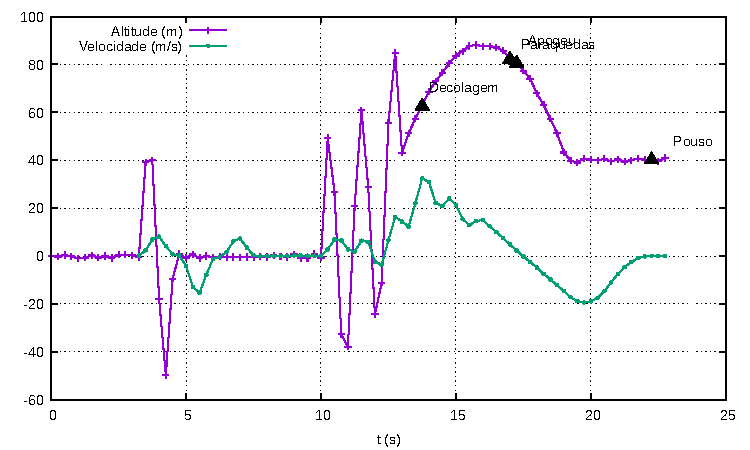
\includegraphics[width=\textwidth]{./data/cases/case05/trajectory}
	\caption{Aplicação dos critérios de detecção de eventos de voo. Caso 5}
	\label{fig:case05}
\end{figure}
\begin{figure}[!ht]
	\centering
	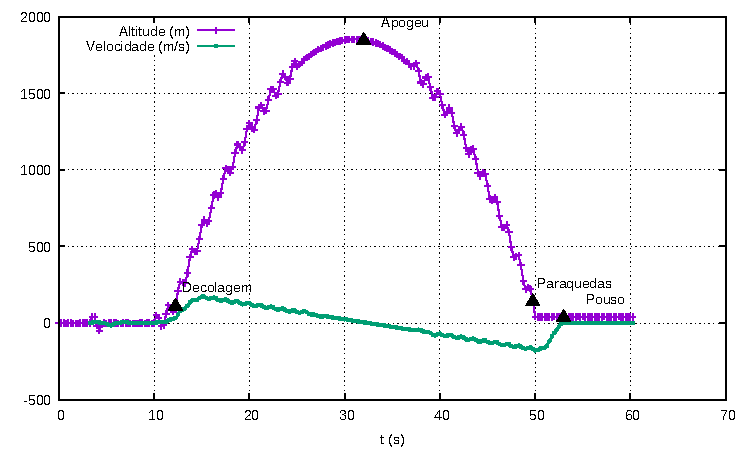
\includegraphics[width=\textwidth]{./data/cases/case06/trajectory}
	\caption{Aplicação dos critérios de detecção de eventos de voo. Caso 6}
	\label{fig:case06}
\end{figure}

\begin{figure}[!ht]
	\centering
	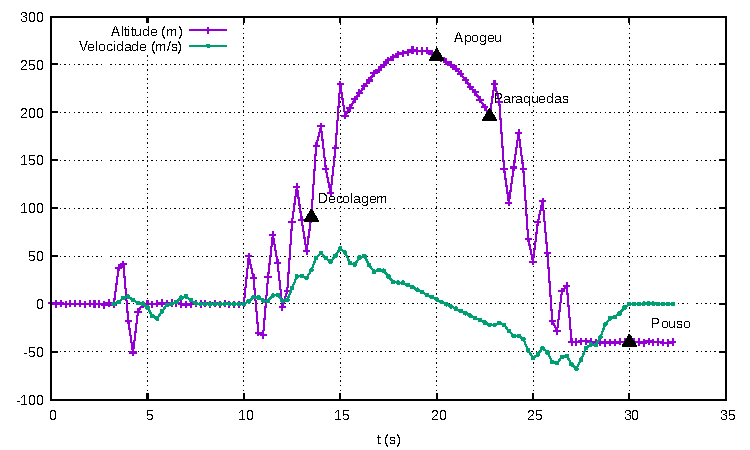
\includegraphics[width=\textwidth]{./data/cases/case07/trajectory}
	\caption{Aplicação dos critérios de detecção de eventos de voo. Caso 7}
	\label{fig:case07}
\end{figure}
\begin{figure}[!ht]
	\centering
	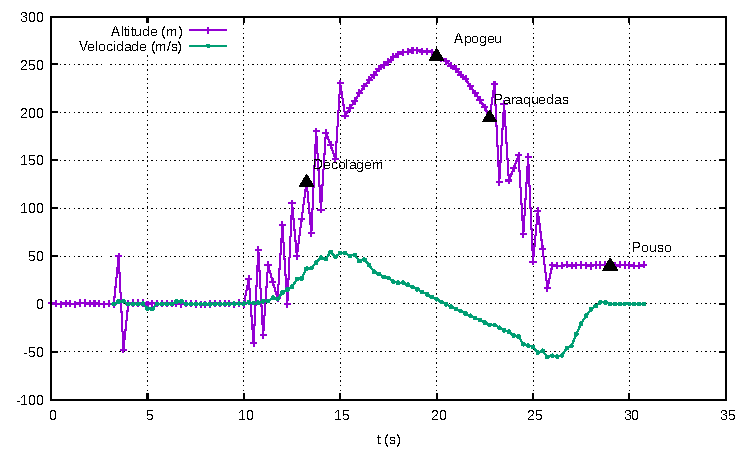
\includegraphics[width=\textwidth]{./data/cases/case08/trajectory}
	\caption{Aplicação dos critérios de detecção de eventos de voo. Caso 8}
	\label{fig:case08}
\end{figure}
\begin{figure}[!ht]
	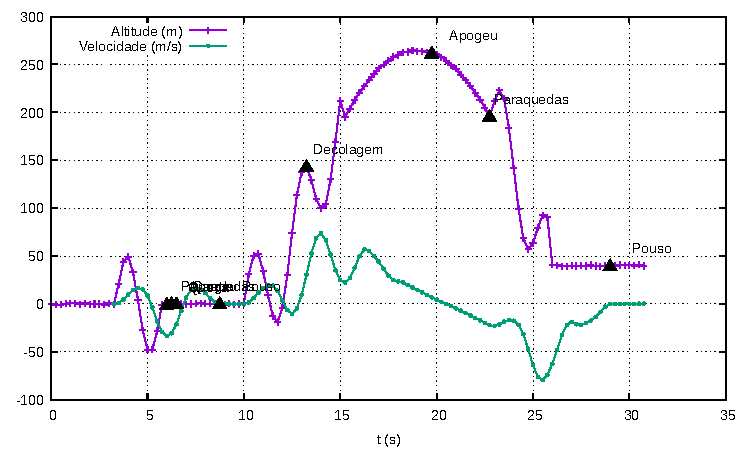
\includegraphics[width=\textwidth]{./data/cases/case09/trajectory}
	\caption{Aplicação dos critérios de detecção de eventos de voo. Caso 9}
	\label{fig:case09}
\end{figure}
\begin{figure}[!ht]
	\centering
	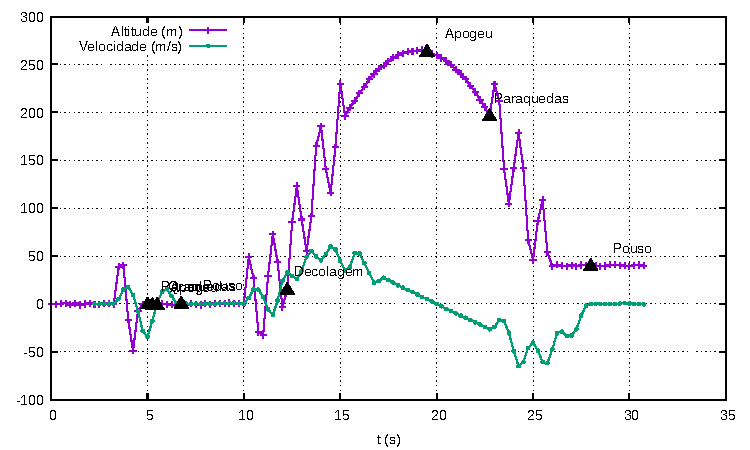
\includegraphics[width=\textwidth]{./data/cases/case10/trajectory}
	\caption{Aplicação dos critérios de detecção de eventos de voo. Caso 10}
	\label{fig:case10}
\end{figure}
\begin{figure}[!ht]
	\centering
	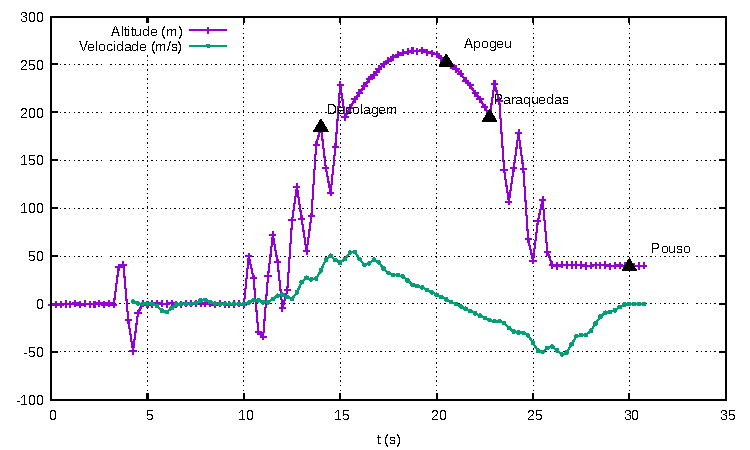
\includegraphics[width=\textwidth]{./data/cases/case11/trajectory}
	\caption{Aplicação dos critérios de detecção de eventos de voo. Caso 11}
	\label{fig:case11}
\end{figure}
\begin{figure}[!ht]
	\centering
	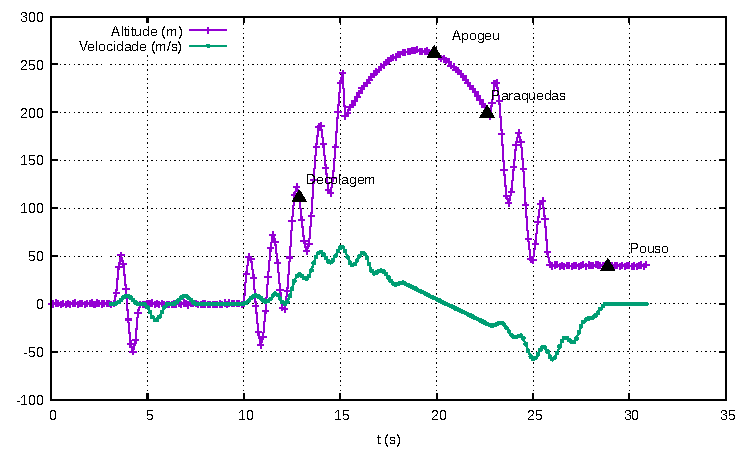
\includegraphics[width=\textwidth]{./data/cases/case12/trajectory}
	\caption{Aplicação dos critérios de detecção de eventos de voo. Caso 12}
	\label{fig:case12}
\end{figure}
\begin{figure}[!ht]
	\centering
	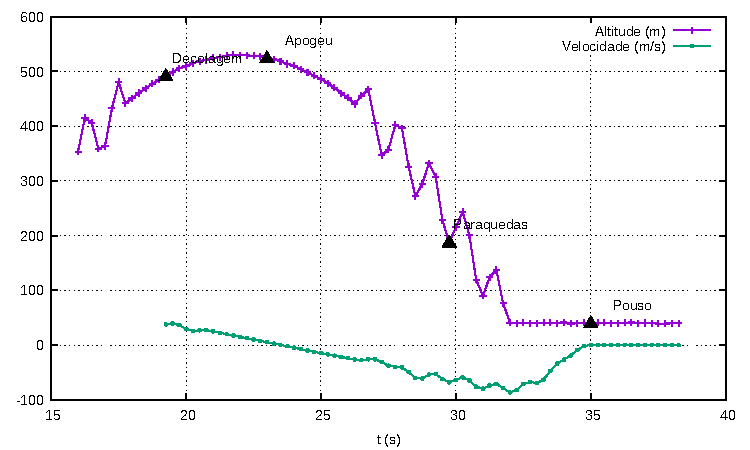
\includegraphics[width=\textwidth]{./data/cases/case13/trajectory}
	\caption{Aplicação dos critérios de detecção de eventos de voo. Caso 13}
	\label{fig:case13}
\end{figure}
\begin{figure}[!ht]
	\centering
	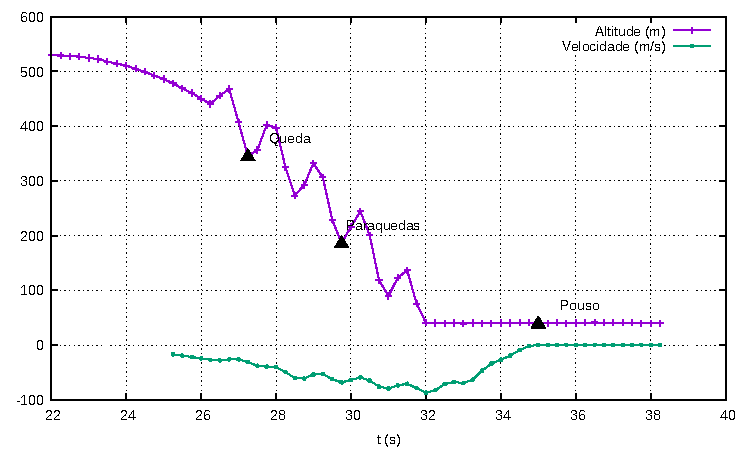
\includegraphics[width=\textwidth]{./data/cases/case14/trajectory}
	\caption{Aplicação dos critérios de detecção de eventos de voo. Caso 14}
	\label{fig:case14}
\end{figure}



\begin{figure}[!ht]
	\centering
	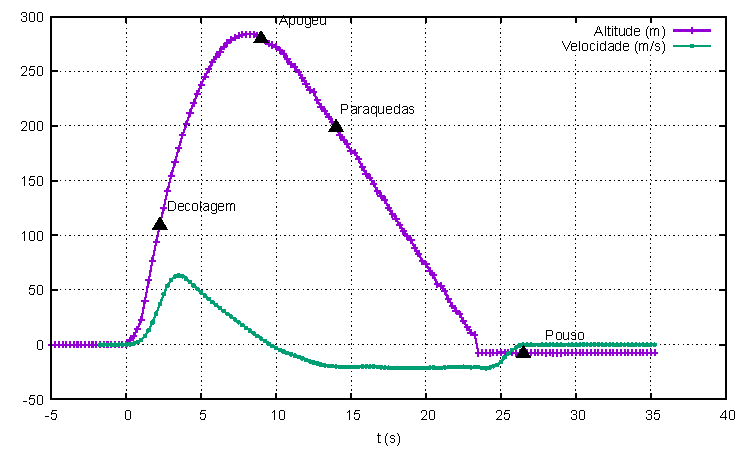
\includegraphics[width=\textwidth]{./data/lacamentos-def-criterios/lancamento01/trajectory}
	\caption{Aplicação dos critérios de detecção de eventos de voo para dados de voos reais. Lançamento  1}
	\label{fig:lancamento01}
\end{figure}
\begin{figure}[!ht]
	\centering
	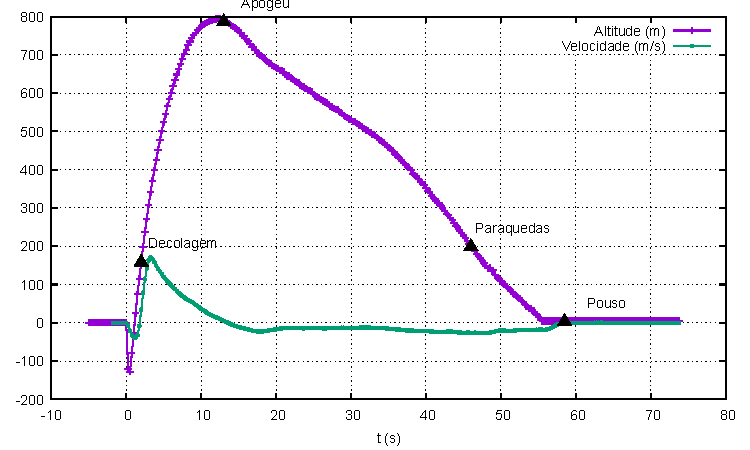
\includegraphics[width=\textwidth]{./data/lacamentos-def-criterios/lancamento02/trajectory}
	\caption{Aplicação dos critérios de detecção de eventos de voo para dados de voos reais. Lançamento  2}
	\label{fig:lancamento02}
\end{figure}
\begin{figure}[!ht]
	\centering
	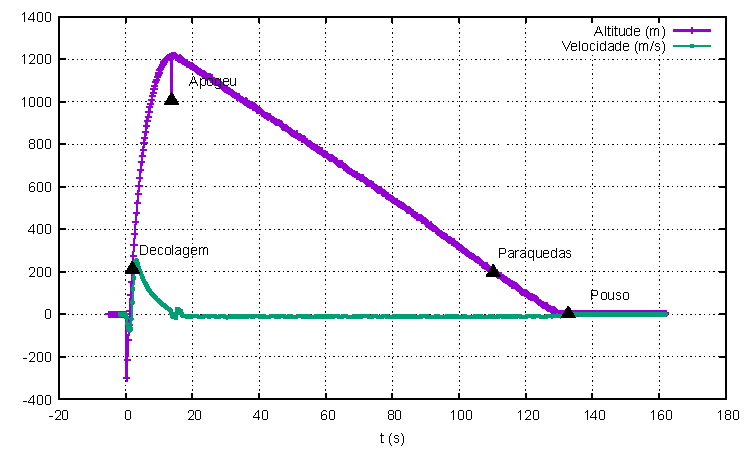
\includegraphics[width=\textwidth]{./data/lacamentos-def-criterios/lancamento03/trajectory}
	\caption{Aplicação dos critérios de detecção de eventos de voo para dados de voos reais. Lançamento  3}
	\label{fig:lancamento03}
\end{figure}
\begin{figure}[!ht]
	\centering
	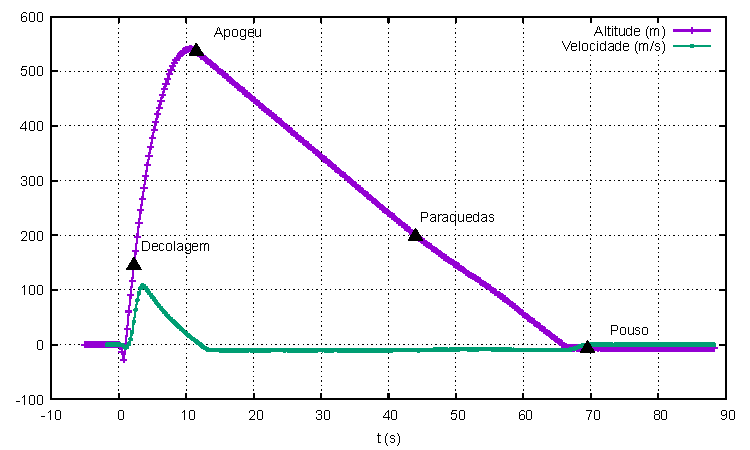
\includegraphics[width=\textwidth]{./data/lacamentos-def-criterios/lancamento04/trajectory}
	\caption{Aplicação dos critérios de detecção de eventos de voo para dados de voos reais. Lançamento  4}
	\label{fig:lancamento04}
\end{figure}
\begin{figure}[!ht]
	\centering
	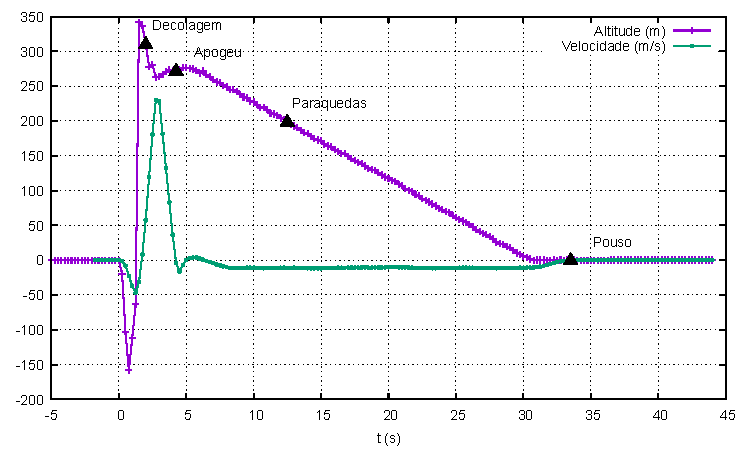
\includegraphics[width=\textwidth]{./data/lacamentos-def-criterios/lancamento05/trajectory}
	\caption{Aplicação dos critérios de detecção de eventos de voo para dados de voos reais. Lançamento  5}
	\label{fig:lancamento05}
\end{figure}
\begin{figure}[!ht]
	\centering
	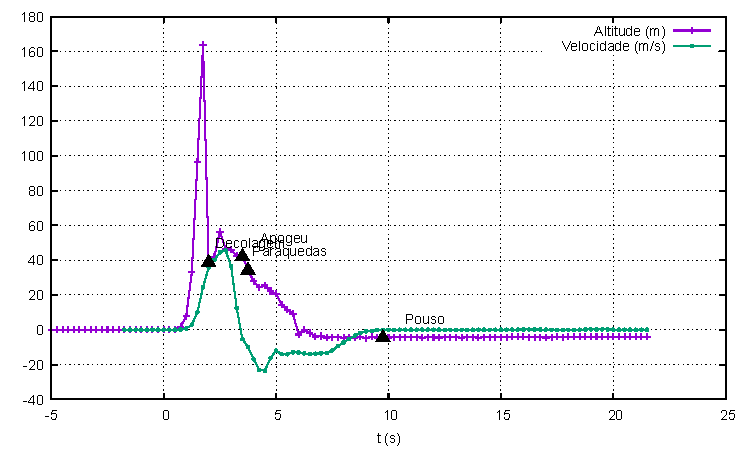
\includegraphics[width=\textwidth]{./data/lacamentos-def-criterios/lancamento06/trajectory}
	\caption{Aplicação dos critérios de detecção de eventos de voo para dados de voos reais. Lançamento  6}
	\label{fig:lancamento06}
\end{figure}
\begin{figure}[!ht]
	\centering
	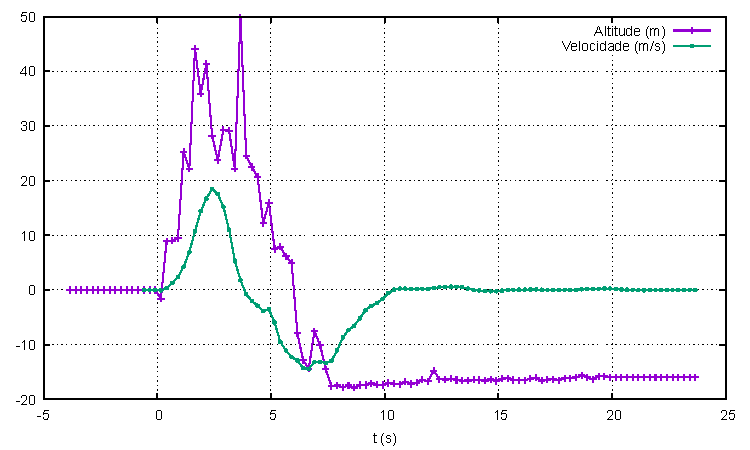
\includegraphics[width=\textwidth]{./data/lacamentos-def-criterios/lancamento07/speedForLiftoffDetection30/trajectory}
	\caption{Aplicação dos critérios de detecção de eventos de voo para dados de voos reais. Lançamento  7 ($\bar{v}_\text{liftoff}=30$~m/s)}
	\label{fig:lancamento07-30}
\end{figure}
\begin{figure}[!ht]
	\centering
	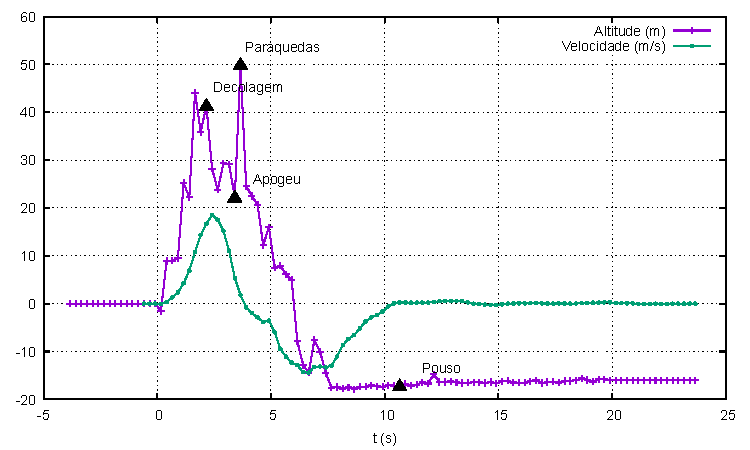
\includegraphics[width=\textwidth]{./data/lacamentos-def-criterios/lancamento07/speedForLiftoffDetection15/trajectory}
	\caption{Aplicação dos critérios de detecção de eventos de voo para dados de voos reais. Lançamento  7 ($\bar{v}_\text{liftoff}=15$~m/s)}
	\label{fig:lancamento07-15}
\end{figure}




\begin{figure}[!ht]
	\centering
	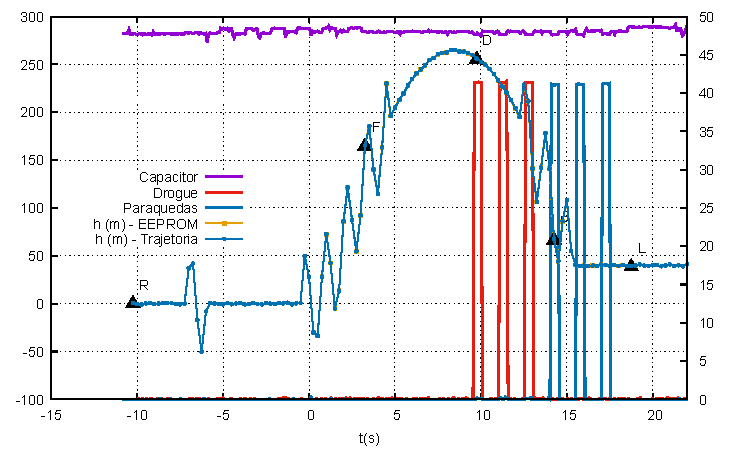
\includegraphics[width=\textwidth]{./data/simulations-v1.5.5/sim01/fig}
	\caption{Testes com barômetro simulado.  Simulação 1}
	\label{fig:sim01}
\end{figure}
\begin{figure}[!ht]
	\centering
	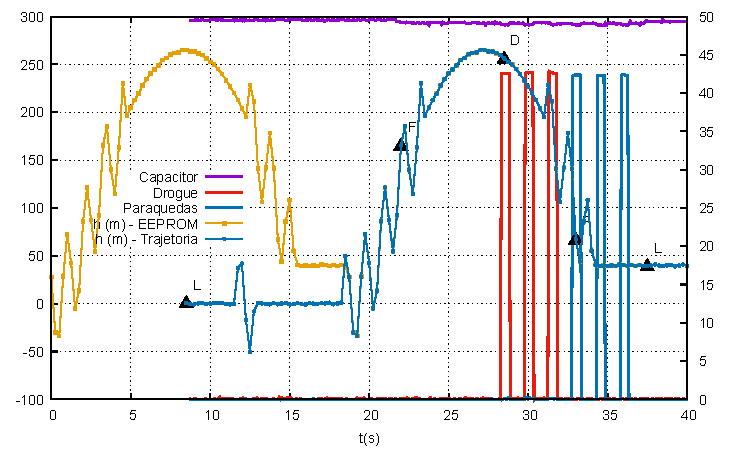
\includegraphics[width=\textwidth]{./data/simulations-v1.5.5/sim02/fig}
	\caption{Teste com barômetro simulado.  Simulação 2}
	\label{fig:sim02}
\end{figure}
\begin{figure}[!ht]
	\centering
	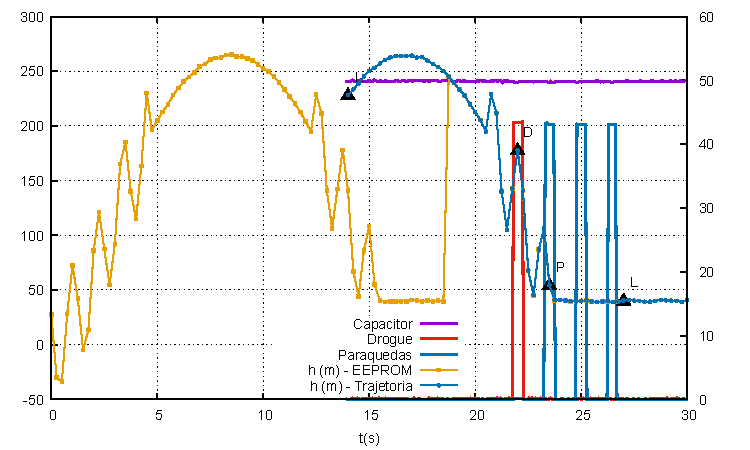
\includegraphics[width=\textwidth]{./data/simulations-v1.5.5/sim03/fig}
	\caption{Teste com barômetro simulado.  Simulação 3}
	\label{fig:sim03}
\end{figure}
\begin{figure}[!ht]
	\centering
	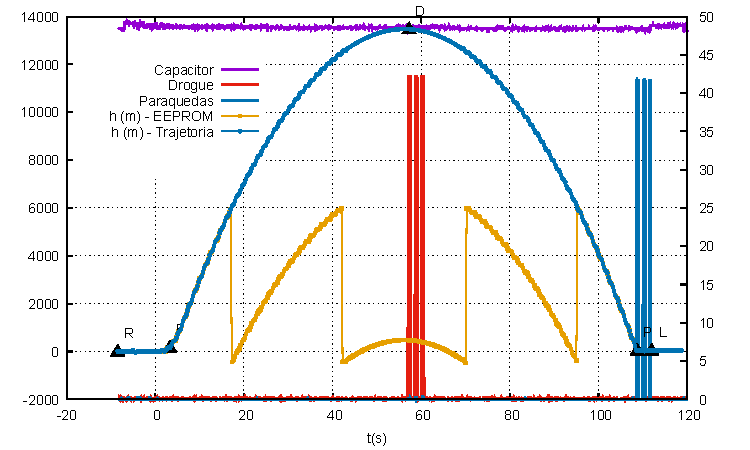
\includegraphics[width=\textwidth]{./data/simulations-v1.5.5/sim04/fig}
	\caption{Teste com barômetro simulado.  Simulação 4}
	\label{fig:sim04}
\end{figure}
	
\begin{figure}[!ht]
	\centering
	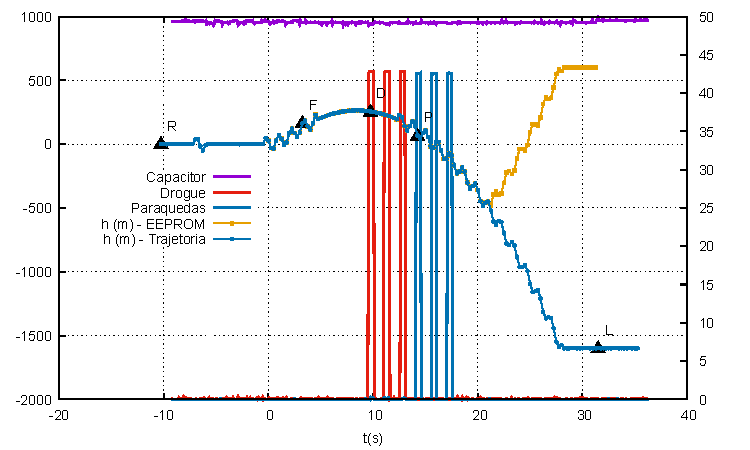
\includegraphics[width=\textwidth]{./data/simulations-v1.5.5/sim05/fig}
	\caption{Teste com barômetro simulado.  Simulação 5}
	\label{fig:sim05}
\end{figure}
\begin{figure}[!ht]
	\centering
	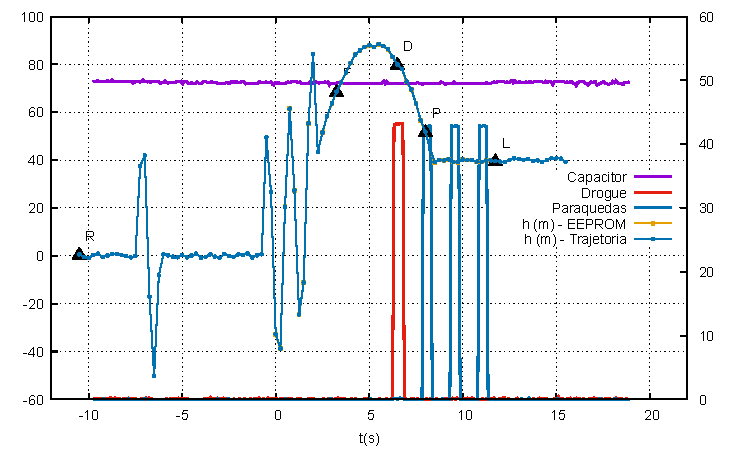
\includegraphics[width=\textwidth]{./data/simulations-v1.5.5/sim06/fig}
	\caption{Teste com barômetro simulado.  Simulação 6}
	\label{fig:sim06}
\end{figure}
\begin{figure}[!ht]
	\centering
	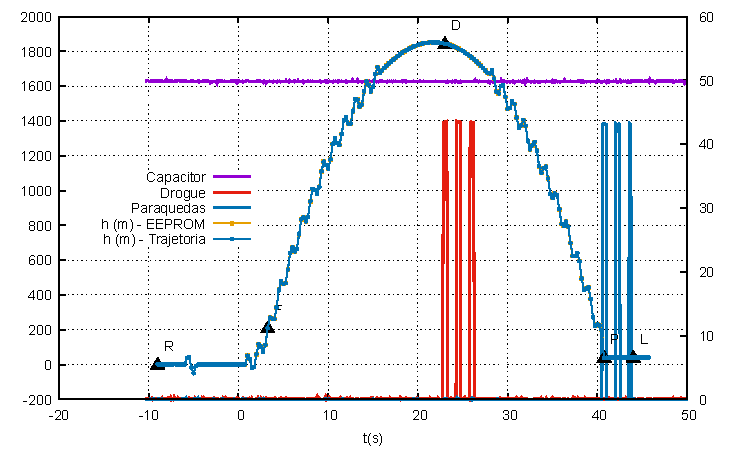
\includegraphics[width=\textwidth]{./data/simulations-v1.5.5/sim07/fig}
	\caption{Teste com barômetro simulado.  Simulação 7}
	\label{fig:sim07}
\end{figure}
\begin{figure}[!ht]
	\centering
	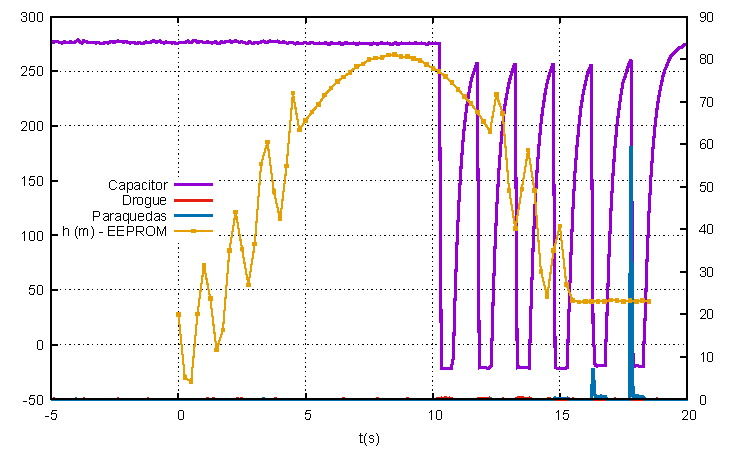
\includegraphics[width=\textwidth]{./data/simulations-v1.5.5/sim08/fig}
	\caption{Teste com barômetro simulado.  Simulação 8}
	\label{fig:sim08}
\end{figure}
\begin{figure}[!ht]
	\centering
	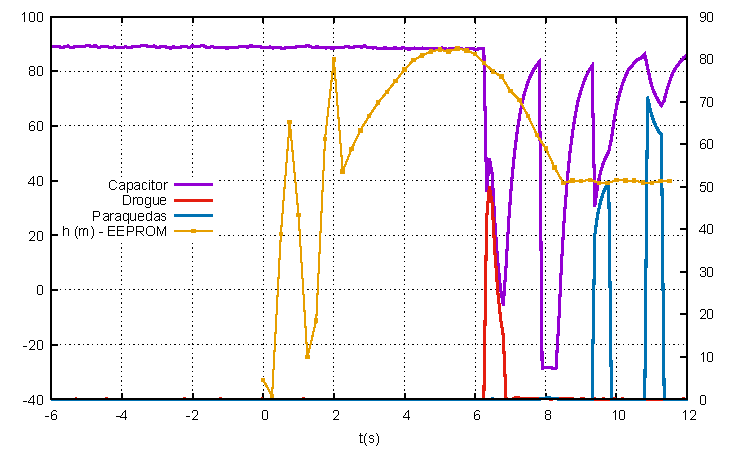
\includegraphics[width=\textwidth]{./data/simulations-v1.5.5/sim09/fig}
	\caption{Teste com barômetro simulado.  Simulação 9}
	\label{fig:sim09}
\end{figure}

\begin{figure}[!ht]
	\centering
	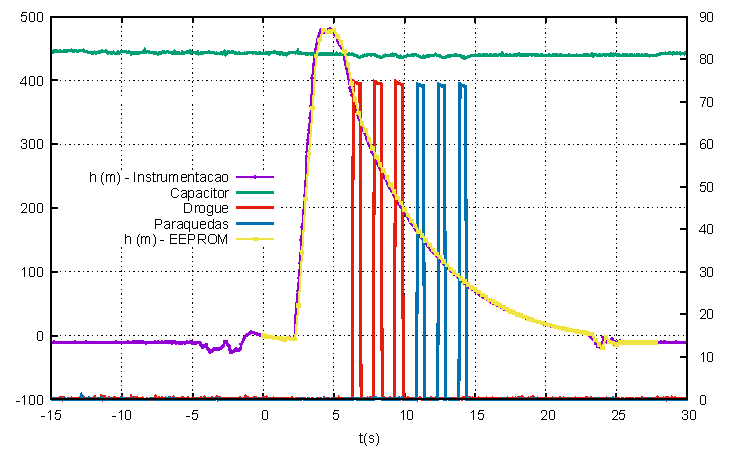
\includegraphics[width=\textwidth]{./data/exp-v1.5.5/exp01/fig}
	\caption{Experimento de bancada  1}
	\label{fig:exp01}
\end{figure}
\begin{figure}[!ht]
	\centering
	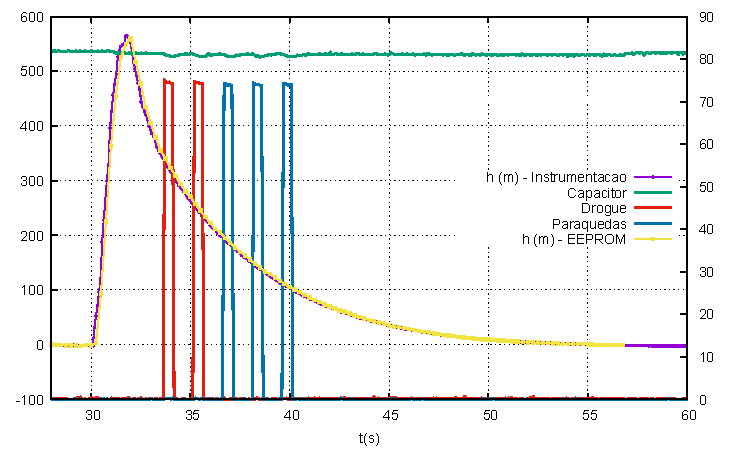
\includegraphics[width=\textwidth]{./data/exp-v1.5.5/exp02/fig}
	\caption{Experimento de bancada  2}
	\label{fig:exp02}
\end{figure}
\begin{figure}[!ht]
	\centering
	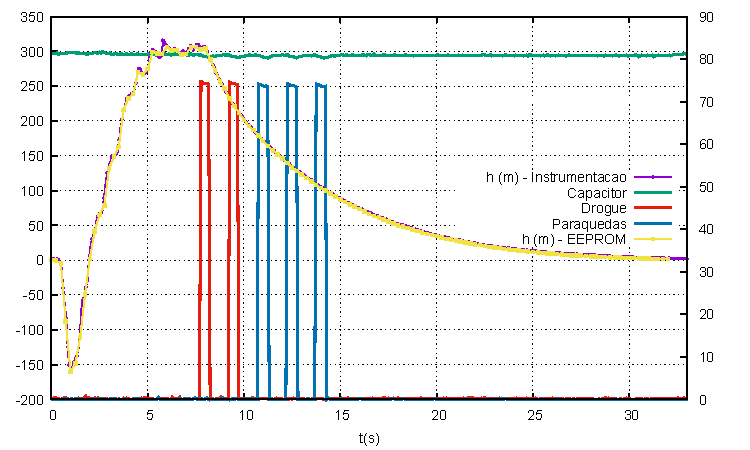
\includegraphics[width=\textwidth]{./data/exp-v1.5.5/exp03/fig}
	\caption{Experimento de bancada  3}
	\label{fig:exp03}
\end{figure}
\begin{figure}[!ht]
	\centering
	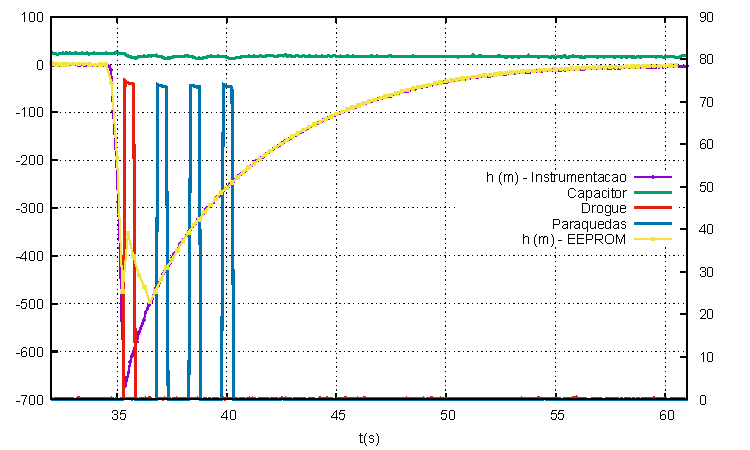
\includegraphics[width=\textwidth]{./data/exp-v1.5.5/exp04/fig}
	\caption{Experimento de bancada  4}
	\label{fig:exp04}
\end{figure}
\begin{figure}[!ht]
	\centering
	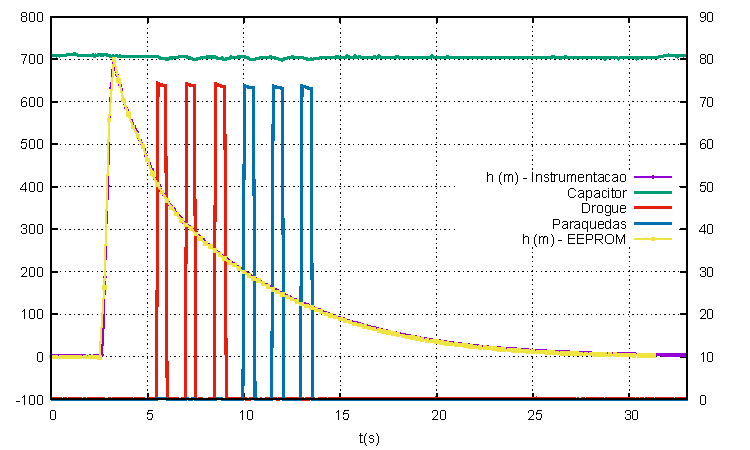
\includegraphics[width=\textwidth]{./data/exp-v1.5.5/exp05/fig}
	\caption{Experimento de bancada  5}
	\label{fig:exp05}
\end{figure}
\begin{figure}[!ht]
	\centering
	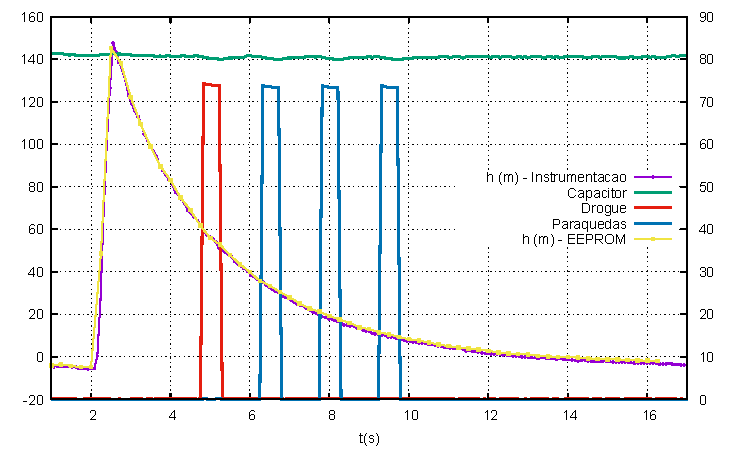
\includegraphics[width=\textwidth]{./data/exp-v1.5.5/exp06/fig}
	\caption{Experimento de bancada  6}
	\label{fig:exp06}
\end{figure}
\begin{figure}[!ht]
	\centering
	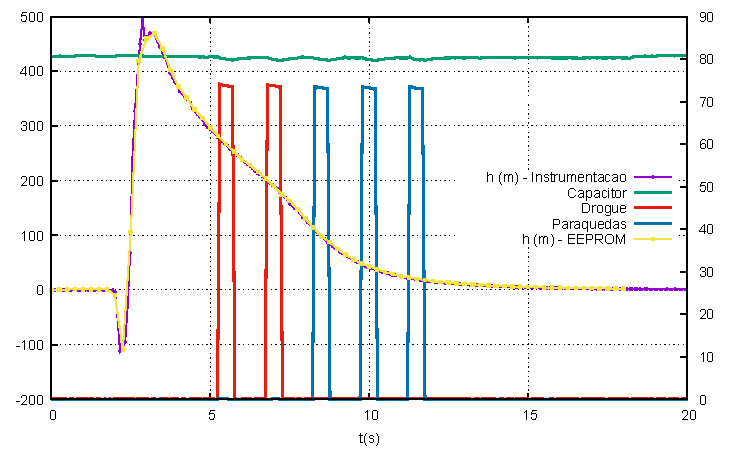
\includegraphics[width=\textwidth]{./data/exp-v1.5.5/exp07/fig}
	\caption{Experimento de bancada  7}
	\label{fig:exp07}
\end{figure}

\end{document}